\documentclass[12pt,a4paper,twoside,openright]{ociamthesis}  % default square logo 
\usepackage[utf8]{inputenc}
%enhanced support of Computer Modern fonts
\usepackage{lmodern}
%additional American Mathematical Society mathematical typesetting capabilities
\usepackage{amsmath}
%American Mathematical Society mathematical theorems
\usepackage{amsthm}
%American Mathematical Society mathematical symbols
\usepackage{amssymb}
% For double line spacing
\usepackage{setspace}
% For opening quote
\usepackage{epigraph}
% For coloured tables
\usepackage[table]{xcolor}
% For rotated table
\usepackage{rotating}
% For nomenclature
\usepackage[intoc]{nomencl}
% For flowchart
\usepackage{tikz}
\usetikzlibrary{shapes,arrows,automata,positioning,fit,calc,backgrounds,chains, decorations.pathreplacing}
% For coloring
\usepackage{color,soul}
% Inline enumeration
\usepackage[inline]{enumitem}

% What was additionally imported by MDPI style
\usepackage{graphicx}
\usepackage{subfig}
\usepackage{multirow}
\usepackage{enumitem}
\usepackage[linesnumbered,lined,boxed,commentsnumbered]{algorithm2e}
\usepackage{footmisc}
\usepackage{etoolbox}
% Fix to allow for \pounds
\usepackage[T1]{fontenc}
% Fix to show \texteuro
\usepackage{textcomp}

%\usepackage[numbers,sort&compress]{natbib}
\usepackage{cite}

\usepackage{array}
\newcolumntype{L}[1]{>{\raggedright\let\newline\\\arraybackslash\hspace{0pt}}m{#1}}
\newcolumntype{C}[1]{>{\centering\let\newline\\\arraybackslash\hspace{0pt}}m{#1}}
\newcolumntype{R}[1]{>{\raggedleft\let\newline\\\arraybackslash\hspace{0pt}}m{#1}}

\usepackage{letltxmacro}
\AtBeginDocument{
  \LetLtxMacro\Oldincludegraphics\includegraphics
%  \renewcommand{\includegraphics}[2][]{\Oldincludegraphics[width=0.9\textwidth,#1]{#2}}
  \renewcommand{\includegraphics}[2][]{%
	\ifstrempty{#1}{%
	  \Oldincludegraphics[width=0.95\textwidth]{#2}%
	}{%
	  \Oldincludegraphics[#1]{#2}%
	}%
  }
%  \renewcommand{\includegraphics}\@ifnextchar[{\@specificincludegraphics}{\@defaultincludegraphics}
%  \cmd\@specificincludegraphics[#1]#2{{\Oldincludegraphics[#1]{#2}}
%  \cmd\@defaultincludegraphics#1{{\Oldincludegraphics[width=0.9\textwidth]{#1}}
}
%\newcommand{\includefig}[1]{\includegraphics[width=0.9\textwidth]{#1}}

\setlength\epigraphrule{0pt}
\renewcommand{\epigraphflush}{center}
\setlength{\epigraphwidth}{0.95\textwidth}

% Change default figure positioning
\makeatletter
  \providecommand*\setfloatlocations[2]{\@namedef{fps@#1}{#2}}
\makeatother
\setfloatlocations{figure}{htbp}
\setfloatlocations{table}{htbp}

%% This code creates the groups
% -----------------------------------------
\renewcommand\nomgroup[1]{%
	\ifthenelse{\equal{#1}{G}}{\item[\textbf{Acronyms}]}{%
		\ifthenelse{\equal{#1}{H}}{\item[\textbf{Definition variables and dimensionality}]}{%
			\ifthenelse{\equal{#1}{I}}{\item[\textbf{Symbols used in Chapter 3}]}{%
				\ifthenelse{\equal{#1}{J}}{\item[\textbf{Symbols used in Chapter 4}]}{%
					\ifthenelse{\equal{#1}{K}}{\item[\textbf{Symbols used in Chapter 5}]}{%
						\ifthenelse{\equal{#1}{L}}{\item[\textbf{Symbols used in Chapter 6}]}{%
							{}}}}}}}}
% -----------------------------------------

% Generate the nomenclature (includes glossary)
\makenomenclature


\title{Service Restoration Algorithm in \\[1ex]
 Distribution Networks by using\\[1ex] Reinforcement Learning}
%note \\[1ex] is a line break in the title

\author{Pablo Alejandro Parra Gómez}
\college{Faculty of Engineering}

%\renewcommand{\submittedtext}{change the default text here if needed}
\degree{Electrical Engineering}
\degreedate{2020}


% end the preamble and start the document
\begin{document}
  %\tracingonline1\tracinggroups1

  % this baselineskip gives sufficient line spacing for an examiner to easily
  % markup the thesis with comments
  \baselineskip=18pt plus1pt

  % set the number of sectioning levels that get number and appear in the contents
  \setcounter{secnumdepth}{3}
  \setcounter{tocdepth}{3}

  \maketitle                  % create a title page from the preamble info
  \doublespacing

  \begin{romanpages}       % start roman page numbering
    %\setlength{\topmargin}{-.5in}

% \epigraph{\textit{It is not a dream. It is a simple feat of scientific electrical engineering. 
% Electric power can drive the world's machinery without the need of coal, oil or gas.
% Although perhaps humanity is not yet sufficiently advanced to be willingly lead by the 
% inventor's keen searching sense. Perhaps it is better in this present world of ours where 
% a revolutionary idea may be hampered in its adolescence. All this that was great in the past 
% was ridiculed, condemned, combatted, suppressed only to emerge all the more triumphantly from 
% the struggle. [...] Our duty is to lay the foundation for those who are to come and to point 
% the way, yes humanity will advance with giant strides. We are whirling through endless space
% with an inconceivable speed, all around everything is spinning, everything is moving,
% everywhere there is energy.}}{--- Nicola Tesla}

\chapter*{Abstract}
\addcontentsline{toc}{chapter}{Abstract}

% give a background
% Summarized the problem 
% State the solution 
% the main aim is to present a methodology for Service Restoration using Reinforcement Learning 
% The proposed Machine Learning technique for solving this problem is Reinforcement Learning 
% Explain the methodology: how is works and what are the constraints preserved 
% How this was tested 

Distribution Networks (DNs) are highly susceptible to faults, which affects their quality and reliability. This thesis proposes a novel Service Restoration approach to help DNs to automatically and intelligently resupply the out-of-service un-faulted customers after a fault occurs. The presented approach is developed with the use of Reinforcement Learning techniques and it is integrated with OpenDSS. 

\vspace*{5ex}
\textbf{\textit{Keywords:}} DA, Reinforcement Learning, Q-Learning, Service Restoration, OpenDSS.

          % include the abstract
    \chapter*{Declaration}
\addcontentsline{toc}{chapter}{Declaration}

I confirm that this is my own work and the use of all material from other sources has been properly and fully acknowledged.

\vspace{5cm}

\noindent\rule{20em}{0.4pt}

Pablo Alejandro Parra Gómez        % declaration of authenticity
    \chapter*{Dedication}
\addcontentsline{toc}{chapter}{Dedication}

I dedicate this work to my family.         % include a dedication.tex file
    \chapter*{Acknowledgments}
\addcontentsline{toc}{chapter}{Acknowledgments}

%I would like to begin by thanking my two B.S. thesis advisors Professor Gustavo Ramos Lopez and Dr. David Celeita Rodriguez for their continuing support, and guidance during this work. 
I would like to thank my advisor Prof. Gustavo Ramos Lopez Ph.D. for his collaboration and guidance during the development of this thesis. Also, for the knowledge acquired throughout the courses.

Besides my advisor, I would like to thank David Celeita Rodriguez Ph.D. for his support and insightful comments.

I would like to express my greatest gratitude to my family. To Cecilia, Lyda, Margarita, Romelia, Myriam, and Hugo for all of their support throughout my life. 
In particular, I would like to thank my mother for her willingness to listen, support, and motivate.

Last but not least, I would like to thank my friends and classmates. 

   % include an acknowledgements.tex file
    \addcontentsline{toc}{chapter}{Table of contents}
    \tableofcontents            % generate and include a table of contents
    \addcontentsline{toc}{chapter}{Table of figures}
    \listoffigures              % generate and include a list of figures

    
\nomenclature[G]{DG}{Distributed Generation}
\nomenclature[G]{DNO}{Distribution Network Operator}
\nomenclature[G]{EPRI}{Electric Power Research Institute}
\nomenclature[G]{IEEE}{Institute of Electrical and Electronics Engineers}
\nomenclature[G]{SAIDI}{System Average Interruption Duration Index}
\nomenclature[G]{SAIFI}{System Average Interruption Frequency Index}
\nomenclature[G]{CAIDI}{Customer Average Interruption Duration Index}
%\nomenclature[G]{ACSs}{Automatic controlled switches}
\nomenclature[G]{SR}{Service Restoration}
\nomenclature[G]{FISR}{Fault Isolation and Service Restoration}
\nomenclature[G]{DAS}{Distribution Automation System}
\nomenclature[G]{DNA}{Distribution Network Automation}
\nomenclature[G]{NO}{Normally Open}
\nomenclature[G]{NC}{Normally Closed}
\nomenclature[G]{ML}{Machine Learning}
\nomenclature[G]{RL}{Reinforcement Learning}
\nomenclature[G]{MAS}{Multiagent Systems}
\nomenclature[G]{CI}{Customers Interruptions}
\nomenclature[G]{CMI}{Customer Minutes of Interruption}
\nomenclature[G]{DN}{Distribution Network}
    \singlespacing
\printnomenclature[1in]
\doublespacing

\nomenclature[H]{n(A)}{The number of actions}
\nomenclature[H]{RR}{Restoration rate}
\nomenclature[H]{$n(IL)_{pre}$}{The number of isolated loads before restoration}
\nomenclature[H]{$n(IL)_{post}$}{The number of isolated loads after restoration}

  \end{romanpages}
    
  \chapter{Introduction}
\label{ch-introduction}
This work intends to contribute to Distribution Networks to improve power supply quality 
and reliability throughout Service Restoration (SR) methodologies. By reviewing and comparing 
the existing SR methodologies, it is possible to identify the challenges and the limitations 
of the current methodologies, in order to develop a solution that attempts to overcome them.
%Service Resotarion techniques by developing an algorithm that

In Chapter 1, the background and motivation of this work are presented. Additionally, and based on the 
identified challenges for SR improvements in distribution networks, the problem statement 
and research objectives are stated.  

\section{Background and Motivation}
\label{ch-introduction:sec:background}

Distribution Networks (DNs) allow supplying power to customers, and power quality and reliability ensure 
customer satisfaction. However, DNs are highly susceptible to failures, which causes more than 85$\%$ 
of power interruptions \cite{Liu2016}. That results not only in decreasing reliability indices but also in 
economic and social impacts \cite{Zidan2017}.

Therefore, there is a necessity to improve the DNs \cite{Kavousi-Fard2014}, whereby, in recent years, utilities 
invest in Distribution Automation (DA) intending to create a self-healing smart grid in order to improve 
SAIDI, SAIFI, and CAIDI indices \cite{Zidan2017}\cite{Angelo2013} \cite{Madani2015}. 
%maybe explain self-healing 

Distribution Automation (DA) takes advantage of available technologies to automate DN operations and enhance 
its performance \cite{U.S.DepartmentofEnergy2018}, since DNs became more difficult to 
design, manage, and sustain \cite{Madani2015}. Consequently, DA includes automated ways to locate the fault 
and restore the service in an optimized approach such as Fault Location, Isolation, and Service Restoration 
(FLISR) \cite{USDepartmentofEnergy2016} \cite{Liu2016}. 

FLISR operates after a fault detection. Firstly, it locates and isolates the fault as fast as possible. After 
the fault area is isolated, it transfers customers to healthy feeders and restores power supply to them 
\cite{Zidan2017}. Otherwise, customers may experience sustained outages \cite{USDepartmentofEnergy2016}. 

In a program conducted by the U.S. Department of Energy \cite{USDepartmentofEnergy2016}, it was shown that FLISR techniques achieve substantial 
DN operation improvements, such as a reduction in the number of customers interruptions (CI) by 55$\%$, and in 
customer minutes of interruption (CMI) by 53$\%$. \footnote{Average per event for FLISR operations reported by five utilities over one year \cite{USDepartmentofEnergy2016}.}

\begin{figure}
    \centering
	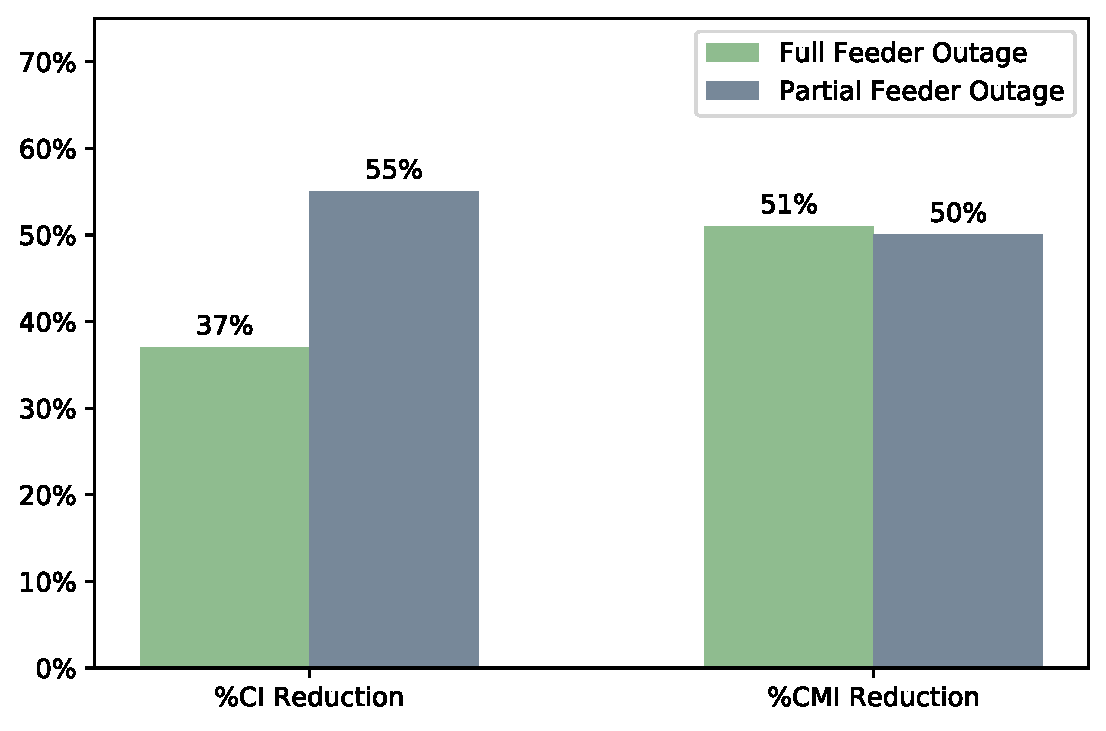
\includegraphics[scale = 0.5]{_introduction/fig/type_outage}
	\caption{FLISR effects on the number of customers interrupted (CI) and customer minutes of interruption (CMI) by the type of outage from USDON2016 \cite{USDepartmentofEnergy2016}.}
	\label{ch-introduction:fig:type_outage}
\end{figure}
\begin{figure}
    \centering
	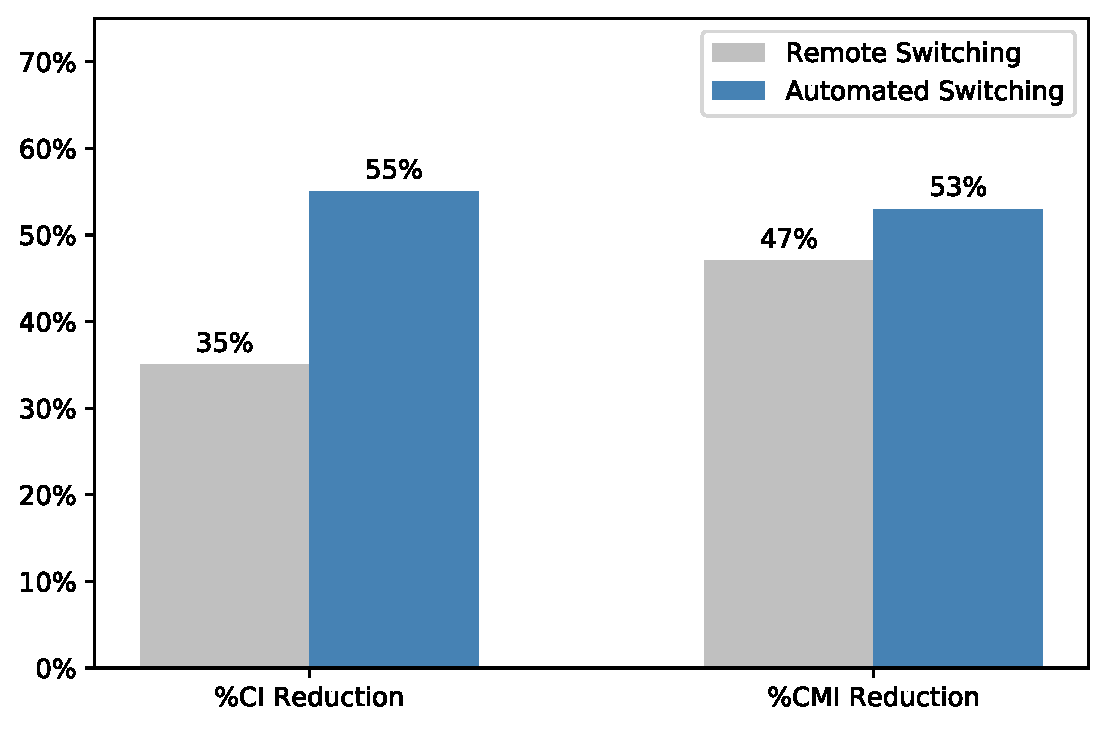
\includegraphics[scale = 0.5]{_introduction/fig/type_scheme.pdf}
	\caption{FLISR effects on the number of customers interrupted (CI) and customer minutes of interruption (CMI) by the type of FLISR operating scheme from USDON2016 \cite{USDepartmentofEnergy2016}.}
	\label{ch-introduction:fig:type_scheme}
\end{figure}

Figures \ref{ch-introduction:fig:type_outage} and \ref{ch-introduction:fig:type_scheme} show the reduction 
in CI and CMI by the type of outage and by type of FLISR scheme, respectively. The first figure states the 
number of customers interrupted decreases by 55$\%$ in a partial feeder outage, while the time of a full 
feeder outage decreases by 51$\%$. On the other hand, the second figure establishes that both CI and CMI 
have a further reduction when the FLISR scheme is automatic. Lastly, it should be pointed out these 
reductions improve directly the reliability indices mentioned before. 

As aforementioned, three stages constitute the FLISR scheme. The last stage is Service Restoration, one of the
most relevant strategies to enhance the resilience of DNs \cite{Shen2018}, and which is the main topic of this work.
%The problem is raised in the next section. 
\section{Problem Statement and Research Objectives}
\label{ch-introduction:sec:problem}

Service Restoration uses network reconfiguration methods to change the DN topology and resupply the out-of-service 
un-faulted customers \cite{Gholami2015}\cite{Shen2018}. This reconfiguration is carried out through 
switching operations, considering typical DNs have normally closed (NC) sectionalizing switches and normally 
opened (NO) tie switches \cite{Zidan2017} \cite{Sanches2014}. I.e., the main goal of SR is to find 
optimal switching sequences for the DN \cite{Latare2017}.

This procedure must maximize the number of loads restored, minimize the number of switching operations, and 
maintain operational and topological constraints \cite{Abu-Elanien2018} \cite{Gholami2015}. 
Nevertheless, and as noted in the formulation problem (Section \ref{ch-literature:sec:overview}), SR is computationally demanding because it is multi-objective, 
non-linear, and operational constrained. And also, it requires to explore a large number of switching operation 
combinations \cite{Shen2018} \cite{Sanches2014}. 

SR algorithm uses one or many techniques to obtain a solution, among which are expert systems, heuristic 
algorithms, meta-heuristic algorithms, graph theory, multi-agent systems, and mathematical programming \cite{Shen2018}. 
Furthermore, they can be implemented under centralized or decentralized approaches \cite{Zidan2017}. The control approaches 
and their corresponding techniques are reviewed, in further detail, in section \ref{ch-literature:sec:overview} and 
summarized in table \ref{ch-introduction:tab:sr_techniques}. 

\begin{table}
    \centering
    \caption{SR techniques comparison \cite{Abu-Elanien2018} \cite{Zidan2017}}
    \label{ch-introduction:tab:sr_techniques}
    \begin{tabular}{|l|c|c|c|}
        \hline
        \multicolumn{1}{|c|}{\textbf{Method}}                                        & \multicolumn{1}{c|}{\textbf{\begin{tabular}[c]{@{}c@{}}Optimal \\ solution\end{tabular}}} & \multicolumn{1}{c|}{\textbf{\begin{tabular}[c]{@{}c@{}}System \\ dependency\end{tabular}}} & \multicolumn{1}{c|}{\textbf{\begin{tabular}[c]{@{}c@{}}Self-learning \\ capacity\end{tabular}}} \\ \hline
        \textbf{Expert systems}                                                      & No                                                                                        & Yes                                                                                       & No                                                                                              \\ \hline
        \textbf{Heuristics}                                                          & No                                                                                        & Yes                                                                                       & No                                                                                              \\ \hline
        \textbf{Meta-heuristics}                                                     & No                                                                                        & Yes                                                                                       & No                                                                                              \\ \hline
        \textbf{\begin{tabular}[c]{@{}l@{}}Mathematical \\ programming\end{tabular}} & Yes                                                                                       & No                                                                                        & No                                                                                              \\ \hline
        \end{tabular}
\end{table}


Table \ref{ch-introduction:tab:sr_techniques} compares the different methodologies used to develop SR 
algorithms and shows their limitations. Most methodologies cannot obtain an optimal solution, 
but improvements in processing time \cite{Abu-Elanien2018}; thus, the solution optimality is sacrificed to obtain a faster solution. 
On the other hand, these methodologies, except mathematical programming, are system dependent and do not 
have the ability to self-learn, becoming out of date when system variations occur \cite{Zidan2017}.

Therefore, these limitations imply a need for human intervention to update their rules or knowledge bases 
and make the methodologies readapt to the new changes.

\subsection{General Purpose}

According to the previous data, the focus of this work is to develop a scalable Service Restoration algorithm 
capable of self-healing Distribution Networks by automatic learning the optimal sequence of switching 
operations to lead DNs to the best possible state after a fault occurs. Moreover, 
the challenge of automatic learning behavior also includes continuous learning, hence the system is 
constantly exploring to improve the sequence and adapt to changes in the network. Last but not least, 
the optimization objectives and constraints formalized in Chapter \ref{ch-literature} are also taken into account.

This work also aims to develop a validation system of the SR algorithm, which allows simulations of a 
practical distribution network and verification of its operational and topological constraints, 
through the integration of a co-simulation engine. 

\begin{enumerate}[
    labelindent=*,
    style=multiline,
    leftmargin=*,
    label=\textbf{Objective~\arabic*}]
        %\item Review existing methods for Service Restoration. 
        %\item Design a solution that improve the existing methods. 
        \item Develop a Service Restoration algorithm for Distribution Networks capable of self-learning to obtain an optimal solution that accomplishes operational and topological constraints by implementing a Reinforcement Learning technique.
        \item Develop a validation system that emulates and measures the parameters of a Distribution Network, in order to test the proposed SR algorithm performance, by integrating a co-simulation engine.
        %\item Develop a validation system by using co-simulation engine. 
\end{enumerate}
    




%This work intends to contribute to Service Resotarion techniques by developing an algorithm that improves the quality and reliability of distribution networks. By implementing Reinforcement Learning to create an agent capable of learning the best reconfiguration scheme feasible without violating DN constraints.As discussed in this thesis, Service Restoration. why is it important. However, successfully combining Machine Learning Techniques to reconfigure distribution networks is still an open research challenge.

  \chapter{Literature Review}
\label{ch-literature}

% revisar \cite{Shen2018}
\section{Overview}
\label{ch-literature:sec:overview}

Many authors have referred and researched the importance of Distribution Automation (DA), and its 
advantages, to improve the quality and reliability of Distribution Networks \cite{Zidan2017} 
\cite{Yao2018} \cite{Abu-Elanien2018} \cite{Madani2015}. 

One of the goals of DA is to obtain a self-healing network capable of 
automatically removing temporary faults throughout the restoration of the un-faulted areas, 
which provides benefits to both utilities and customers. Utilities will improve their reliability 
indices and their profits because they reduce penalties from regulators and costs of restoration. 
In addition, customers will obtain a more reliable and continuous power supply \cite{Angelo2013}. 

This self-healing network can be achieved with SR methodologies 
\cite{USDepartmentofEnergy2016} \cite{Yokoyama2012} \cite{Koch-Ciobotaru2014} \cite{Zidan2012}.

\section{Service Restoration}
\label{ch-literature:sec:sr}
Service Restoration can be performed by centralized and decentralized approaches \cite{Zidan2017}\cite{Yip2017}.
The first one includes expert systems, heuristics, metaheuristics, and mathematical programming methodologies; 
the second relies on Multiagent Systems (MAS) \cite{Chellaswamy2019}. 

The two types of approaches, and their corresponding methodologies, are reviewed in section \ref{ch-literature:sec-sr:approaches}. 
However, both approaches tend to solve the Service Restoration problem that can be 
formalized as a general optimization problem, as suggested in section \ref{ch-literature:sec-sr:problem_formulation}. 


\subsection{General SR Problem Formulation}
\label{ch-literature:sec-sr:problem_formulation}
Service Restoration can be formalized as an optimization problem \cite{Huang2016}. 

The main objective function aims to maximize the number of loads restored (equation 
\ref{ch-introduction:equ:max_loads}), while the second aims to minimize the number of operations performed 
to resupply the aforementioned loads (equation \ref{ch-introduction:equ:min_ops}) \cite{Shen2018}. 

\begin{equation} 
\text{max} \sum_{i=1}^{n} L_i \cdot k_i
	\label{ch-introduction:equ:max_loads}
\end{equation}
where $L_i$ is the load at bus \textit{i}, and $k_i$ is its status (1: restored; 0: not restored).
\begin{equation} 
    \text{min } n_{ops} 
    \label{ch-introduction:equ:min_ops}
    \end{equation}
where $n_{ops}$ is the number of switching operations. 

\subsubsection*{Constraints}
The presented objective functions are subject to operational and topological constraints \cite{Abu-Elanien2018}. 

\begin{enumerate}
    \item \textbf{Radial topology:} Radial network topology should be preserved.
    \item \textbf{Bus voltage limits:} Nodal voltage $V_i$ should be within the minimum $V_{min}$ and maximum $V_{max}$ voltage limit: $V_{min} \leq V_i \leq V_{max}$ 
    \item \textbf{Line current limits:} Line current $I_i$ should be under the maximum acceptable line current $ I_{max}$: $I_i \leq I_{max}$.
\end{enumerate}

\subsection{Control approaches and methodologies}
\label{ch-literature:sec-sr:approaches}
\subsubsection*{Centralized approach}
The centralized approach is the principal control approach used in Service Restoration \cite{Abu-Elanien2018}. 
It captures and processes measurements and status information of the entire distribution network to obtain 
an optimal 
SR solution \cite{Koch-Ciobotaru2014}, because of that it requires an extensive computational capacity and a low latency system 
communication \cite{Zidan2017} \cite{Shen2018}. 
Nonetheless, the communication system can be a single point of failure \cite{Shen2018}. 

Among its methodologies are expert system, heuristics, metaheuristic, and mathematical programming 
\cite{Chellaswamy2019}. 



\begin{enumerate}
    \item \textbf{Expert system:} creates rules relying on expert knowledge \cite{Shen2018}. 
    It is a successful way to SR, however, its solution depends on the system and does not guarantee 
    optimality. Besides, its maintenance is expensive for large networks \cite{Zidan2017} \cite{Shen2018}. 
    \item \textbf{Heuristics:} partition and approximate the SR problem by 
    using expert knowledge to obtain a feasible solution. Heuristics present an improvement in time 
    processing, but a difficulty to obtain an optimal solution \cite{Abu-Elanien2018}\cite{Shen2018}. 
    \item \textbf{Mathematical programming:} is a direct method to address the SR optimization problem 
    by obtaining an optimal solution. Although, it demands substantial processing time for large networks
    \cite{Abu-Elanien2018}. 
    \item \textbf{Metaheuristics:} solves the SR problem as an optimization problem, as well as Mathematical Programming (MP),  
    but with less processing time than MP and with a better solution than Heuristics \cite{Abu-Elanien2018}. 
    This is performed by simplifying a problem with many objectives into a problem with a single equivalent objective \cite{Shen2018}. 
     However, the processing time is still huge for practical networks \cite{Zidan2017}. 
\end{enumerate}

\subsubsection*{Decentralized approach}
Decentralized approach distributes the intelligence across the distribution network \cite{Shen2018}, as opposed 
to unique control intelligence in the centralized approach. This structure requires a more robust 
and reliable communication system, but it overcomes the centralized approach disadvantages of huge 
computational capacity and one single point of failure \cite{Zidan2017} \cite{Abu-Elanien2018}. However, since in this approach, the 
agent does not know all the distribution network but its neighbor network, the solution 
obtained is suboptimal \cite{Koch-Ciobotaru2014}. 
This approach is implemented through Multiagent Systems (MAS). 


Figure \ref{ch-literature:tab:control_appraches} summarizes the strengths and limitations of each of the approaches discussed above.
\begin{table}
\centering
\caption{Service Restoration Control approaches}
\label{ch-literature:tab:control_appraches}
\begin{tabular}{|l|l|l|}
\hline
\textbf{Approach}      & \textbf{Strengths}                                                       & \textbf{Limitations}                                                                       \\ \hline
\textbf{Centralized}   & \begin{tabular}[c]{@{}l@{}}- Optimal solution \\ \end{tabular}          & \begin{tabular}[c]{@{}l@{}}- Huge computing capacity\\ - Single point of failure\end{tabular} \\ \hline
\textbf{Decentralized} & \begin{tabular}[c]{@{}l@{}}- Fast solution \\ - Less data\end{tabular} & \begin{tabular}[c]{@{}l@{}}- Suboptimal solution\\ \end{tabular}                          \\ \hline
\end{tabular}
\end{table}
%\begin{enumerate}
%    \item \textbf{Multiagent systems:}
%\end{enumerate}

%centralized

%computes the global optimal
%reconfiguration of the grid, considering all the constraints and using measurements 
%and status information for all across the grid.
%\cite{Koch-Ciobotaru2014}

%requires knowledge of the entire structure of the system
%\cite{Koch-Ciobotaru2014}

%the main control approach for reconfiguration problem
%Most of the existing studies adopted a centralized control approach
%\cite{Abu-Elanien2018}


%low latency communication system to 
%requires/transfer large/huge amounts of data among field agents and control centers (low latency)
%\cite{Zidan2017} \cite{Chellaswamy2019} \cite{Shen2018}

%thus requiring enormous/expensive computational capacity
%\cite{Chellaswamy2019} \cite{Shen2018}

%centralized methods suffer from a single point failure risk
%\cite{Zidan2017} \cite{Shen2018}

%Heuristic, metaheuristic, expert system, and mathematical solutions
%\cite{Chellaswamy2019}

% -------------------------
%expert systems 
%transfers the expert knowledge into some rules

%the maintenance of a large-scale ES is very costly and the optimality of the solution cannot be guaranteed
%\cite{Shen2018}

%The expert system approach is considered a successful way to solve SR problems; however, maintenance of large-scale expert systems has turned out to be costly. Moreover, expert system rules are system-specific, and changed with system variations
%\cite{Zidan2017}

%heuristics
%While heuristic algorithms can obtain a feasible solution
%quickly, they still require specialists’ knowledge and it is hard to derive an optimal solution.
%\cite{Shen2018}

%approaches require extensive computational time when applied for practical distribution systems
%\cite{Zidan2017}

%The meta-heuristic algorithms take less time than mathe-
%matical programming to solve the problem especially in large systems. However, the computational 
%time still considerable in case of large systems. Moreover, the data structure may affect the
%computational time of the meta-heuristic algo- rithms. Poorly prepared data structure can increase 
%the com- putational time dramatically. Although the solution of meta-heuristic algorithms is near 
%optimal solution but it is not optimal. Generally, the solution is better than the heuristic solution 
%and is acceptable by many operation engineers.
%\cite{Abu-Elanien2018}

%Meta- heuristic solve the problem based on the mathematical optimization model
%In conventional meta-heuristic algorithms , a multi- objective problem is converted into an
%equivalent single objective problem by weighting factors, and the admissible switching sequence 
%is not given
%\cite{Shen2018}

%\textbf{Descentralized}

%Decentralized approaches are based on direct peer-to-peer communication between monitoring devices
%\cite{Zidan2017}

%the multi- agent system (MAS) is developed to distribute the intelligence and control actions
% to the component level
%\cite{Shen2018}

%decentralized approach has the advantage of computation speed as it computes a local optimal s
%olution for the grid reconfiguration
%\cite{Koch-Ciobotaru2014}

%Multi-agent systems are systems with multiple interacting elements (agents). Agents are computer 
%systems that are cap- able of deciding what to do in order to satisfy the assigned job to them, 
%and they are also capable of interacting with other agents to perform the overall system goals .

%the necessity of effi- cient and reliable communication system may limit the application 
%of decentralized approaches on full size distribu- tion systems
%suboptimal plan, and this is one of the drawbacks of the decentralized approaches
%\cite{Abu-Elanien2018}

\section{Reinforcement learning}
\label{ch-literature:sec:rl}

Accordingly to the main goal of this work, there is a need to provide the ability of autonomous 
learning to the Service Restoration algorithm, by which it can find the optimal sequence of 
switching operations independently of system variations and without human interventions.
For this reason, Reinforcement Learning plays an important role in  the development of the SR algorithm. 


Reinforcement Learning is a machine learning technique between supervised and unsupervised learning. 
It consists of an interaction between an agent and an environment through which the agent learns to achieve 
RL goals, previously defined. This interaction is two-way communication: first, the environment sends its 
current state to the agent; then, the agent chooses an action, based on that state, and returns its decision to the environment. 

Consequently, actions attempt to modify the environment (i.e., an agent selects the action, and the environment executes it) 
which changes the previous state and leads to a new one.  
The new state fixes new environment parameters that the environment itself must reward according to 
learning objectives. Additionally, these parameters allow the agent to identify a terminal state. 

As a result, the agent gets an immediate reward on the last action-state 
pair and updates its value based on its value function. It is to be noted that the agent's goal is to 
maximize the reward, and the value function depends on the selected RL algorithm, among which are Dynamic Programming, 
Monte Carlo, Q-learning, Sarsa, and Dyna Q.

The theory presented in this section is based on the work conducted by Sutton and Barto \cite{Sutton2014}. 

\subsection{Q-learning}
Q learning is one of the Temporal Difference algorithms. It learns directly from experience and 
updates its value function after each interaction, due to it combines the best features 
of both Monte Carlo and Dynamic Programming methods. 

This tabular RL algorithm saves the action-state value estimates in an $m$ by $n$ matrix, where $m$ 
represents the number of states and $n$ the number of actions, so each position corresponds to an 
action-state value.  After each interaction, the agent updates the corresponding action-state 
value by using Equation \ref{ch-literature:equ:q_value} \cite{Sutton2014}. 
\begin{equation}
Q(S_t, A_t) = Q(S_t, A_t) + \alpha \cdot [R_{t+1} + \gamma \cdot max_a Q(S{t+1,a}) - Q(S_t, A_t)]
\label{ch-literature:equ:q_value}
\end{equation}

  \chapter{Service Restoration Algorithm}
\label{ch1}

The present chapter describes each block of the Service Restoration Algorithm proposed in this study. 

\section{Overview}
\label{ch1:sec:overview}

The algorithm contains two parts:  a training scenario and a production scenario.
Both implement Reinforcement Learning and have a co-simulation engine. 
However, the first one co-simulates with OpenDSS via COM interface and does not have 
prior knowledge about the distribution network; while, the second one co-simulates 
with OpenDSS-G through TCP/IP protocol and does know the distribution network dynamics. 
The co-simulation engine differs from scenarios due to performance.
OpenDSS-G adds a graphic user interface which helps to visualize the topology of the 
distribution network and its changes, but also adds more processing time compared with OpenDSS. 

The SR algorithm is written in Python 3.7 and has an Objet Oriented Programming structure.
Also, it requires the following input data from the distribution network: lines, switches, 
the state of the switches, bus voltages, line currents, load powers, and incidence matrix. 

According to this, Figure \ref{ch1:fig:rl_scenarios} presents the general SR algorithm block diagram.

\begin{figure}
    \centering
    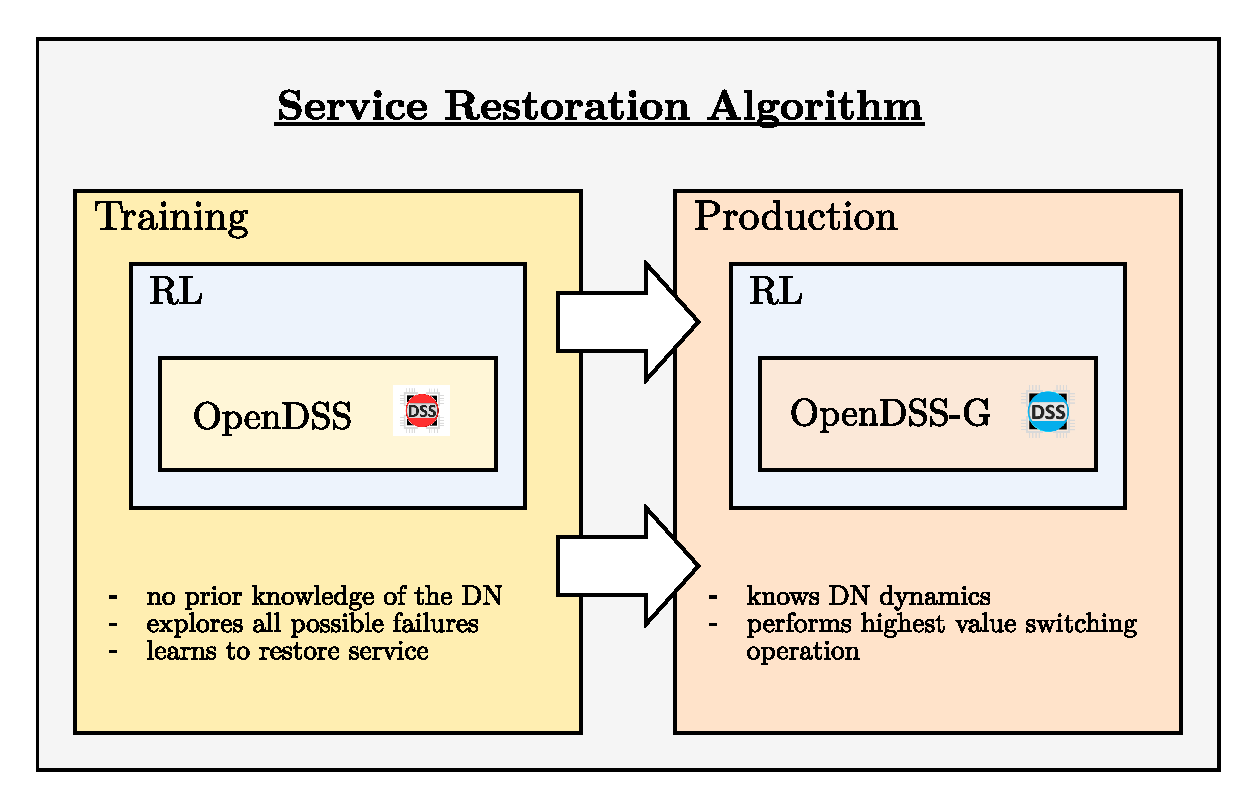
\includegraphics[scale=0.6]{_chapter1/fig/rl_scenarios.pdf}
    \caption{RL scenarios}
    \label{ch1:fig:rl_scenarios}
\end{figure}
\section{Reinforcement Learning implementation}
\label{ch1:sec:reinforcement}

Two components support the Reinforcement Learning: the environment and the zone agent. 
The first one relates to a distribution network and its elements, whereas the second 
one to a learning agent.

The distribution network is susceptible to failures and switching operations, which modifies 
its topology and operation values. 
On the other hand, the zone agent performs Service Restoration on the environment to learn 
the optimal sequence of switching operations after a failure occurrence. 

Figure \ref{ch1:fig:mdp_blocks} presents the interaction between these two elements, which 
allows the algorithm to learn and to automate the decision-making process. This interaction 
is defined in the next section using a finite Markov Decision Process (MDP).

\begin{figure}
    \centering
    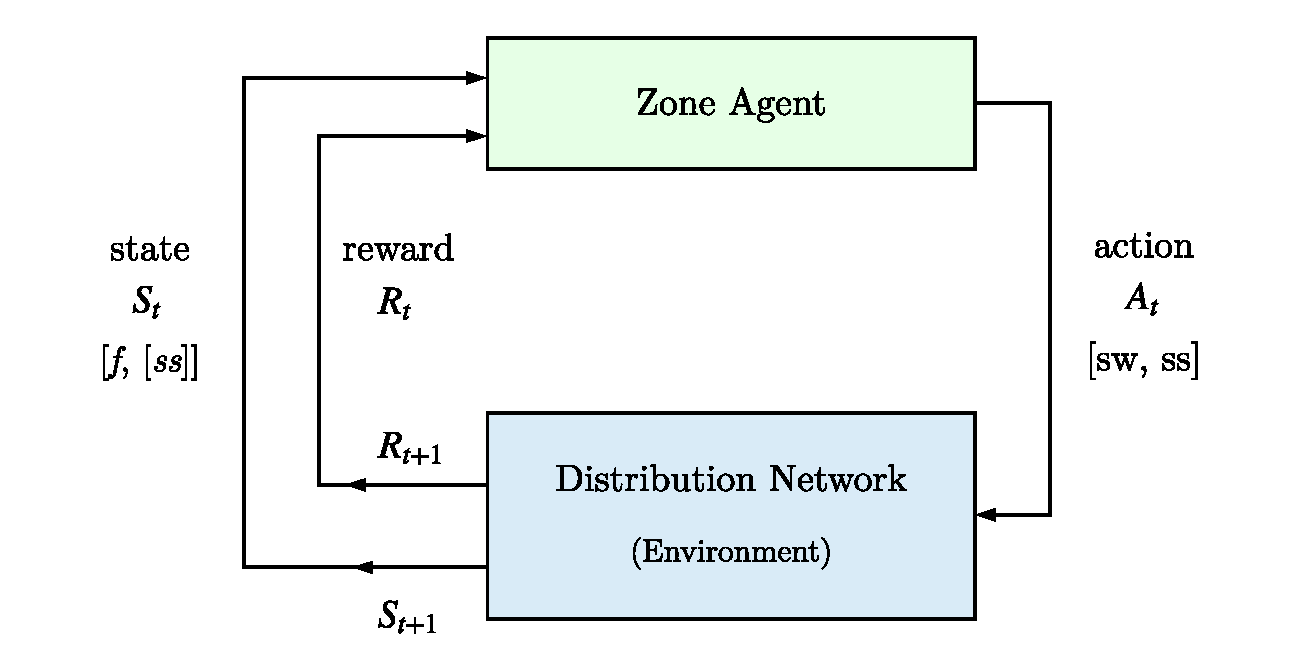
\includegraphics[scale=0.6]{_chapter1/fig/mdp_blocks}
    \caption{MDP block diagram}
    \label{ch1:fig:mdp_blocks}
\end{figure}

\subsection{Markov Decision Process}

MDP is a framework that defines the interaction between the agent and the environment in terms of states,
actions, and rewards. These terms are defined as follows:

\nomenclature[G]{MDP}{Markov Decision Process}

\subsubsection{MDP Elements}

A \textit{state} ($s_t$) defines how the environment is at a particular time and corresponds to an
ordered pair of two elements $[f, [ss]]$. The first element corresponds to a specific failure 
(\textit{f}), while the second one is an ordered list of zeros and ones representing the state of 
switches ($[ss]$). A closed switch takes the value of one, while an open switch takes zero.

Equation \ref{ch1:equ:num_states} returns the total number of states $n(S)$, from the numbers of switch 
status $n(ST)$, switches $n(SW)$, and lines $n(LN)$. 
\begin{equation}
\begin{split}
n(S) &= n(ST)^{n(SW)}*n(LN)\\
\end{split}
\label{ch1:equ:num_states}
\end{equation}

\nomenclature[H]{$n(S)$}{The number of states }
\nomenclature[H]{$n(ST)$}{The number of switch status}
\nomenclature[H]{$n(SW)$}{The number of switches}
\nomenclature[H]{$n(LN)$}{The number of lines}


\nomenclature[H]{$s_t$}{State at time step \textit{t}}
\nomenclature[H]{$[f, [ss]]$}{State: ordered pair of failure and the state of switches}
\nomenclature[H]{\textit{f}}{Failure}
\nomenclature[H]{\textit{$[ss]$}}{The state of switches (ordered list)}

An \textit{action} ($a_t$) is a selection, made by the agent, of which switch operates next. 
However, it does not define the switching operation. The decision if the selected switch opens or 
closes is determined by the opposite of its status, i.e., the agent chooses a switch instead of a 
switching operation. 

\nomenclature[H]{$a_t$}{Action taken at time step \textit{t}}

A \textit{policy} ($\pi$) tells the agent how to take actions from states. It can be 
deterministic or stochastic. 

\nomenclature[H]{$\pi$}{Policy of the Reinforcement Learning algorithm}

A \textit{reward signal} is a numeric value that rates a chosen action, from a given state, 
based on the Service Restoration constraints, e.g., it assigns a negative number for every 
violated restriction.

\subsubsection{MDP Interaction}

\begin{figure}
    \centering
    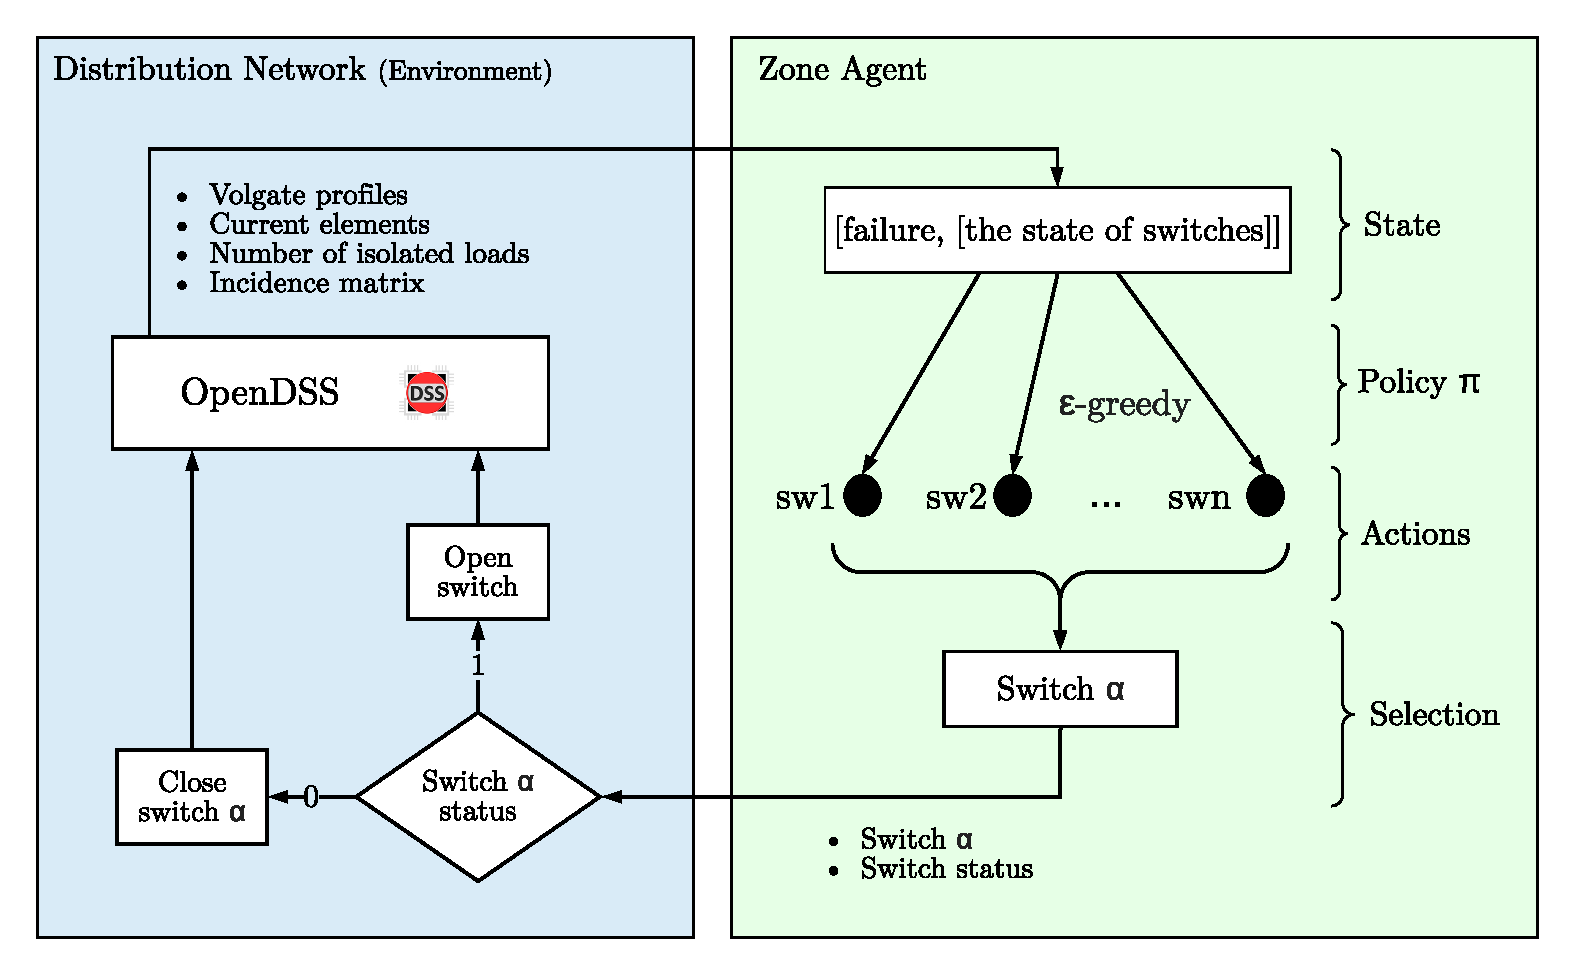
\includegraphics{_chapter1/fig/mdp_blocks_details}
    \caption{MDP block diagram details}
    \label{ch1:fig:mdp_blocks_details}
\end{figure}

A failure occurrence $f$ triggers the interaction between the environment and the agent.
The first to initialize is the environment. It gets its current state $[f,[ss]]$ and sends it to the 
zone agent, who uses it to know which are the possible actions from that state.
Secondly, the zone agent starts and chooses its first switch based on the $\epsilon$-greedy policy.
And then, it sends the switch to the environment, which checks its status and performs the 
corresponding switching operation. 

After the switching operation, the distribution network reaches the next state, which 
drives to new network parameters. These parameters include voltage and current profiles, 
number of isolated loads, and topology. Consequently, the environment compares them 
with the system constraints to verify their fulfillment and, relying on this, rewards 
the state-action pair. 

The reward depends on the number of violated constraints and their hierarchy. For this 
reason, the number of loads isolated receives the highest penalty, followed by voltage and 
current limits, and, lastly, the number of loops within the DN. 

To end the first interaction, the agent gets the reward and the next state and uses them 
to update the value of the previous state-switch pair. The switch-value update depends on 
the RL algorithm implemented. The present study implements two  RL algorithms, which are 
explained in the following section. 

After the action-value update, a new interaction begins, as described above, until the agent 
reaches the terminal state.  As a result, this performs an RL episode. But the agent needs 
hundreds of episodes to learn an optimal policy. 

Figure \ref{ch1:fig:mdp_blocks_details} summarized the details for the proposed MDP.



\subsection{RL episode}
\begin{figure}[!ht]
    \centering
    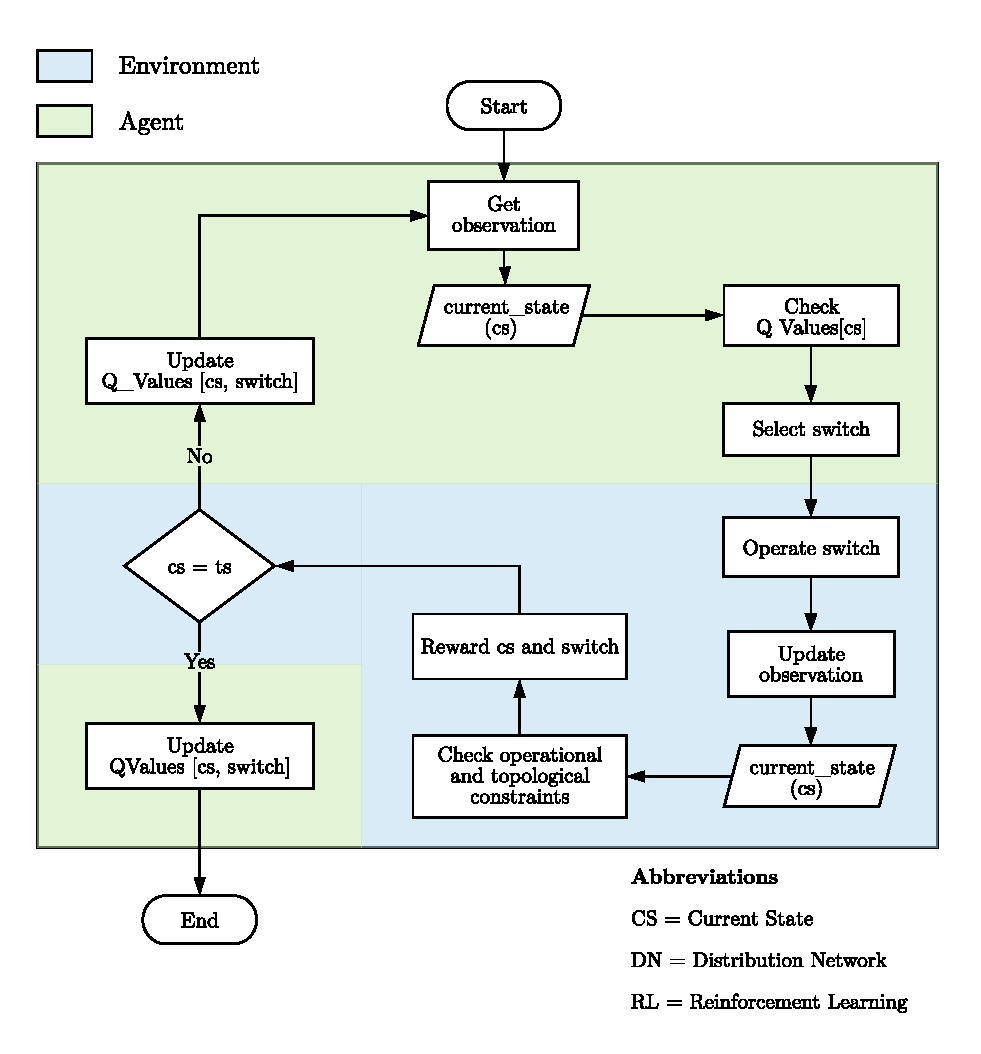
\includegraphics[scale=0.7]{_chapter1/fig/rl_episodes.pdf}
    \caption{Reinforcement Learning Episode}
    \label{ch1:fig:rl_episode_blocks}
\end{figure}

The previous section explains the detail of the MDP interaction between the environment and the agent. Each of those interactions corresponds to an episode. 

Figure \ref{ch1:fig:rl_episode_blocks} shows a block diagram for interaction, but this time from the Service Restoration algorithm perspective. 

%% AP ends ---------------------------

%The interaction starts with the environment initialization which includes a failure occurrence. The environment
%gets its current state $[f, [ss]]$ and sends it to the zone agent, who uses that information to choose a switch. 
%The switch is selected based on an e-greedy policy. The switch selected is sent to the environment, where it performs the switching operation, the switching operation is the opposite of the switch status. Then it collects information about the distribution network, which includes voltage and current profiles, number of isolated loads, and topology.  This data is used to rewards that action. 
%The reward is now sent to the agent with the new current state. The agent updates the value function and takes 
%the next switch. 


%\subsection{Q-learning}

%\subsubsection{Algorithm parameters}

%\subsection{Dyna-Q+}

%\subsubsection{Algorithm parameters}
%A \textit{policy} ($\pi$) says the agent how to take actions from states. The policy also differs from training and 
%production scenarios. The training policy is e-greedy which means that the actions are taken greedy
%1-e percert of the time. While the remaining e percent of the time, the actions are taken ramdonly. 
%This allows the agent to a continuos learning due to the agent explotes when the an action is taken 
%greedy and explore when the action is taken ramdonly. This is valid for training escenario but production 
%scenario, 
% not sure if the policy changes from scenarios 

%A \textit{reward signal} is an immediate sense of how good is the action taken, it takes into account the constrains 
%of the Service Restoration problem. And it assigns a value for every violated restriction. it helps to 
%define the goal of RL. The reward scheme is as follows: 

%Input data 
%In addition to the state, the environment gives the zone agent a package of information about the
%distribution network that includes voltages and currents profiles, number of isolated loads, and
%network topology. 


% que se hace si el espacio de actions y estado no es pequeño, no se puede usar un metodo tabular? 
\section{OpenDSS Co-simulation}
\label{ch1:sec:opendss}

OpenDSS is a fundamental part of the Service Restoration algorithm development. Firstly, it represents the environment in the reinforcement learning model by simulating the entire distribution network. In this way,  it interacts with the agent and performs the switching operations he orders. 

On the other hand, it is the analysis tool that performs power flow calculations in each interaction with the agent. It offers voltage and current profiles, the number of isolated loads, and topology information.

The training scenario uses OpenDSS while production uses OpenDSS-G. The connection with the SR algorithm handles COM interface and TCP/IP, respectively.  

\section{Training scenario}
\label{ch1:sec:training}
\begin{figure}
    \centering
    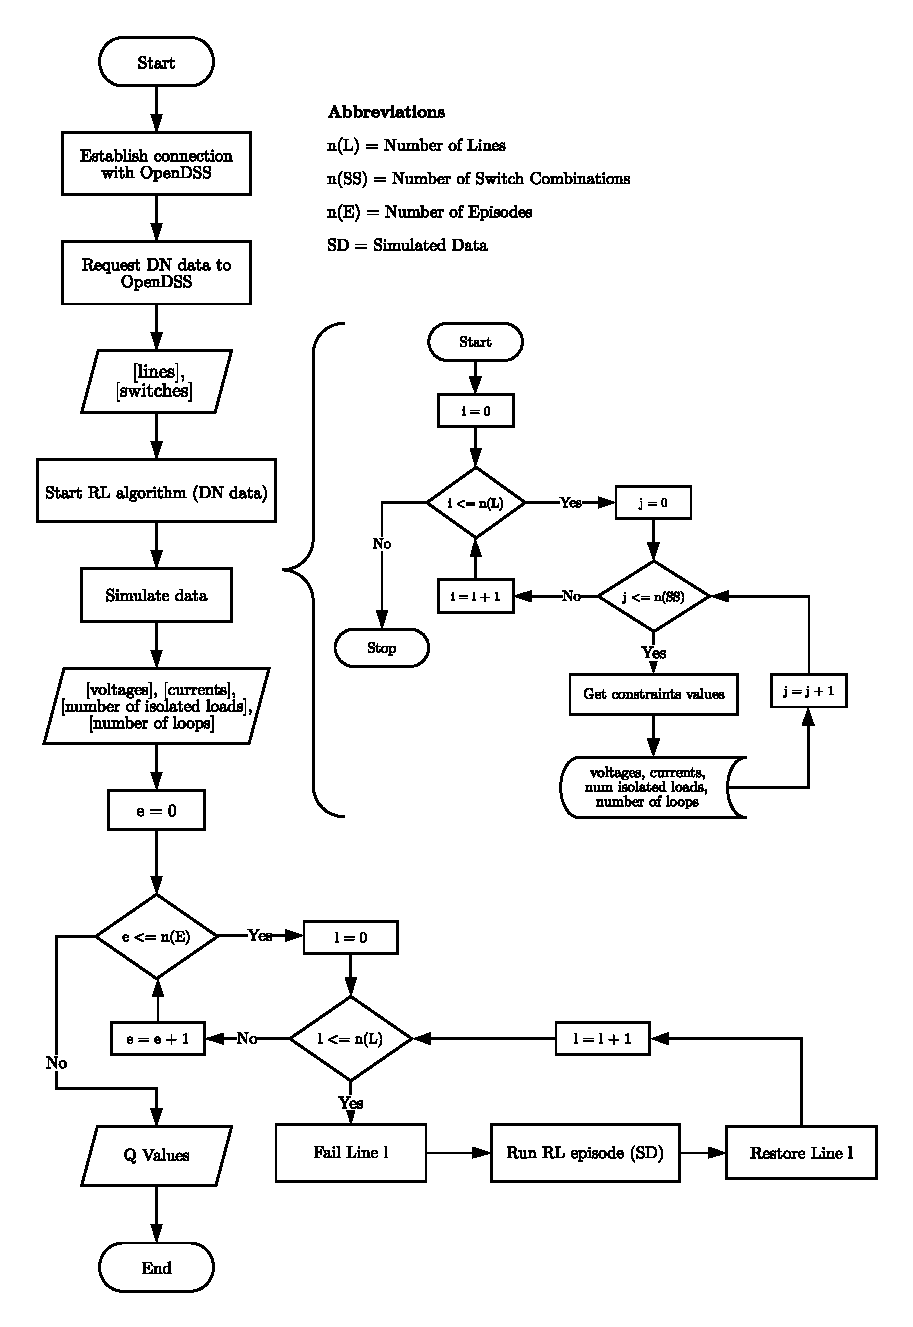
\includegraphics[scale=0.9]{_chapter1/fig/training_scenario.pdf}
    \caption{SR Algorithm - Training Scenario}
    \label{ch1:fig:training_blocks}
\end{figure}

The restoration algorithm starts with Training scenario, which is presented in Figure \ref{ch1:fig:training_blocks}. 
In there, the SR algorithm establishes a connection with OpenDSS and requests the lines and switches data. 
Then, it initializes the RL class with lines and switches passed as a parameter. 

Henceforth, the RL class handles the SR algorithm processes. First, it co-simulates with OpenDSS to obtain the voltage and current profiles, the number of isolated loads, and the number of loops for all possible switch status and faulted line combinations. This simulated data is stored in .ftr files and loaded into the SR algorithm.

Secondly, an episode begins: a line is selected and faulted. So, the RL object performs interactions between the agent and the environment until the environment reaches the terminal state, which is the optimal state after a fault event. 
Once the terminal state is reached, the RL algorithm restores the faulted line and repeats the aforementioned process by selecting a new line to fail. 

This must be done for all lines and during a fixed number of episodes. 

As a result, the Q value matrix stores the optimal SR plan, and the training is completed. 

\section{Production scenario}
\label{ch1:sec:production}

\begin{figure}[!hb]
    \centering
    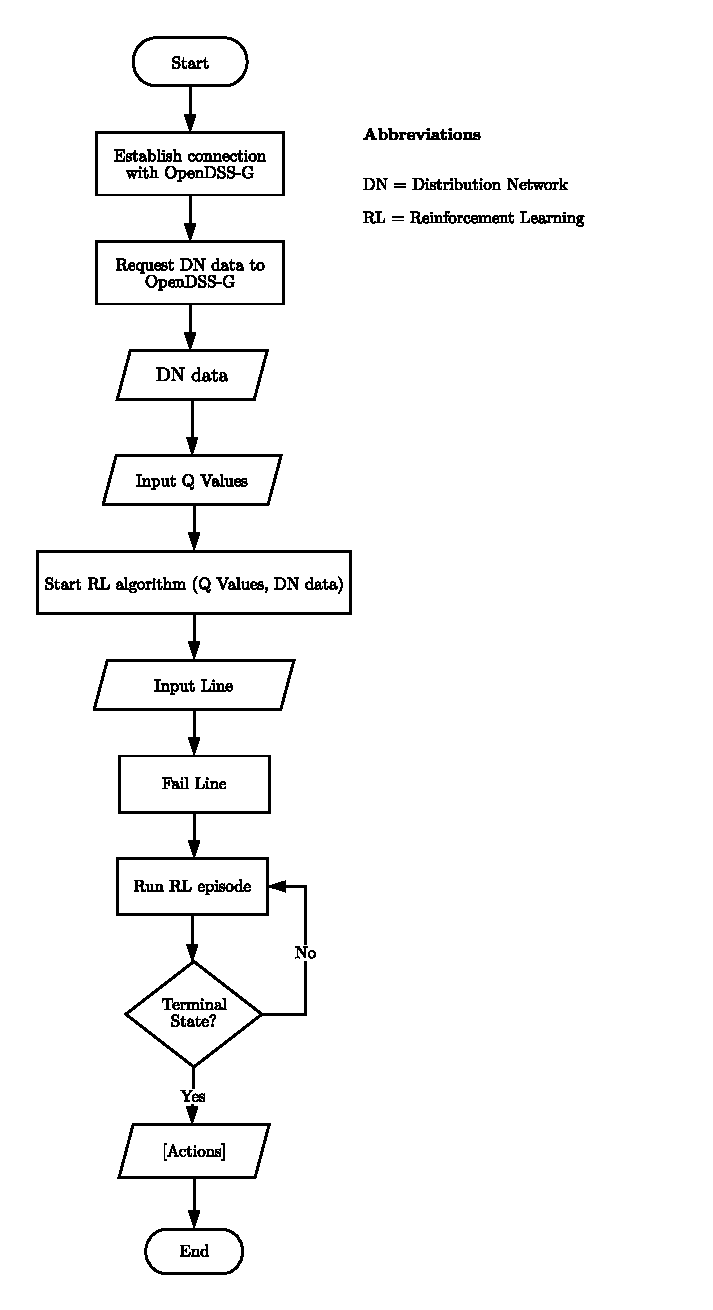
\includegraphics[scale=0.9]{_chapter1/fig/production_scenario.pdf}
    \caption{SR Algorithm - Production Scenario}
    \label{ch1:fig:production_blocks}
\end{figure}

Figure \ref{ch1:fig:production_blocks} shows that Production scenario behaves similarly to Training but with some exceptions. First, the initial 
connection is carried out with OpenDSS-G. Second, the Q Values matrix has been already computed, 
so this scenario aims to apply the Service Restoration plan to lead the network to the best possible 
state after a fault occurrence through self-healing. Third, RL episode runs only once and performs 
just the necessary switching operations until it reaches the terminal state, instead of switching 
operations for all possible faults and switch status combinations. And last, this results in a list 
of actions performed during the SR plan and an updated Q Values matrix. 
  \chapter{Service Restoration Algorithm Validation}
\label{ch2}

\section{Overview}
\label{ch2:sec:overview}

As mentioned before in Chapter 2, the Service Restoration algorithm must execute a Training scenario followed by a Production scenario to obtain a restoration plan. Nevertheless, Training and Production can be carried out independently, although the latter requires the Q Values matrix as input data.

To validate the effectiveness and performance of the SR algorithm, two different Distribution Networks provided by the IEEE Power and Energy Society (IEEE-PES) were tested.

In the following sections, the test cases are presented. 
\section{Test Cases}
\label{ch2:sec:test_cases}
The IEEE Power and Energy Society (IEEE-PES) provides several test cases. The present validation examines and tests the following: 

\subsection{IEEE 33 Node Test Feeder}
Figure \ref{ch2:fig:33bus} shows the IEEE 33 node test feeder topology and Table \ref{ch2:tab:dn_data} summaries its parameters. 
\begin{figure}
    \centering
    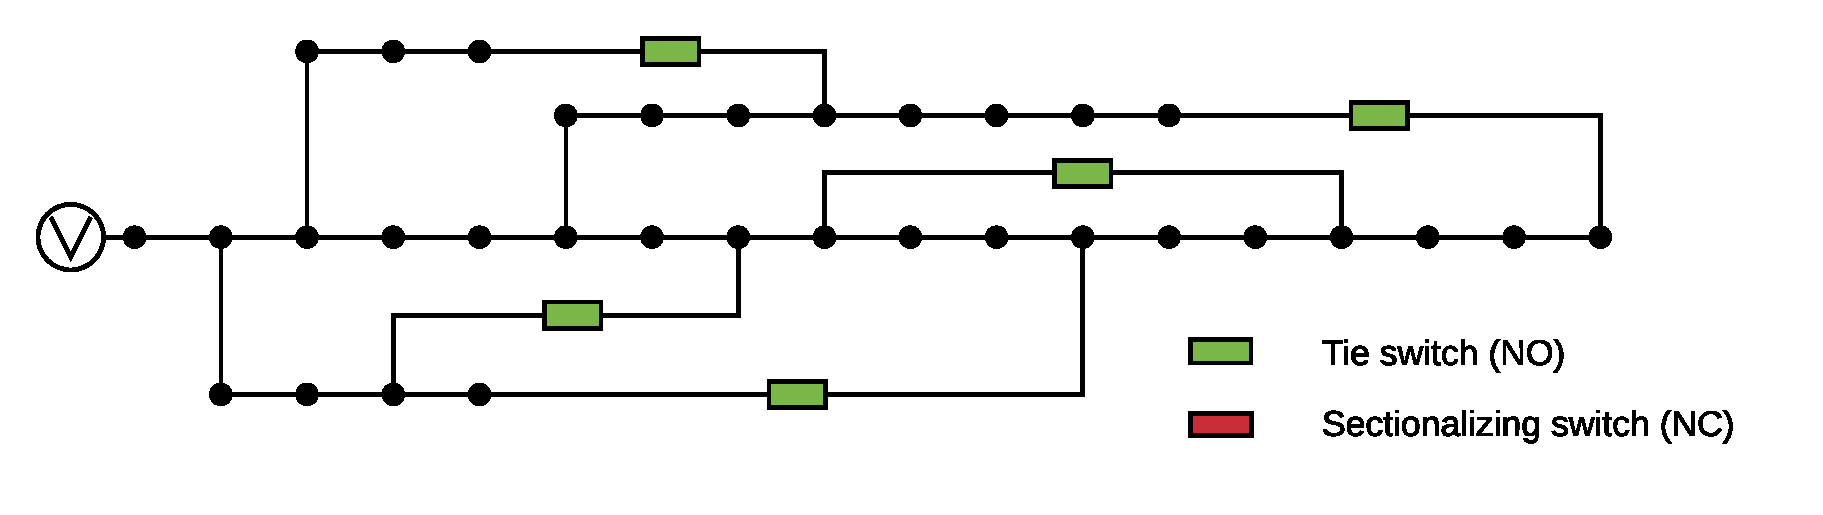
\includegraphics[scale=0.4]{_chapter2/fig/33bus_tc.pdf}
    \caption{IEEE 33 Node Test Feeder from \cite{Landeros2019}}
    \label{ch2:fig:33bus}
\end{figure}

\begin{table}
\centering
\caption{IEEE test feeders data}
\label{ch2:tab:dn_data}
    \begin{tabular}{lcc}
    \hline
    \textbf{DN Elment}         & \textbf{\begin{tabular}[c]{@{}c@{}}33 Node\\ Test Feeder\end{tabular}} & \textbf{\begin{tabular}[c]{@{}c@{}}123 Node \\ Test Feeder\end{tabular}} \\ \hline
    \textit{\textbf{Lines}}    & 32                                                                     & 117                                                                      \\
    \textit{\textbf{Switches}} & 2 - 5                                                                      & 5 - 15                                                                     \\
    \textit{\textbf{Loads}}    & 32                                                                     & 91                                                                      
    \end{tabular}
    \end{table}

\subsection{IEEE 123 Node Test Feeder}

This system is modified to observe the behavior of the Service Restoration Algorithm and to compare 
its performance according to the number of switches. For this reason, they have tested ten variants 
of this test feeder. Each modification increases the number of switches by one, where the minimum is 
five switches and the maximum is fifteen.

Figure \ref{ch2:fig:123bus} shows the IEEE 123 node test feeder topology with 10 switches and 
Table \ref{ch2:tab:dn_data} summaries its parameters. 
\begin{figure}
    \centering
    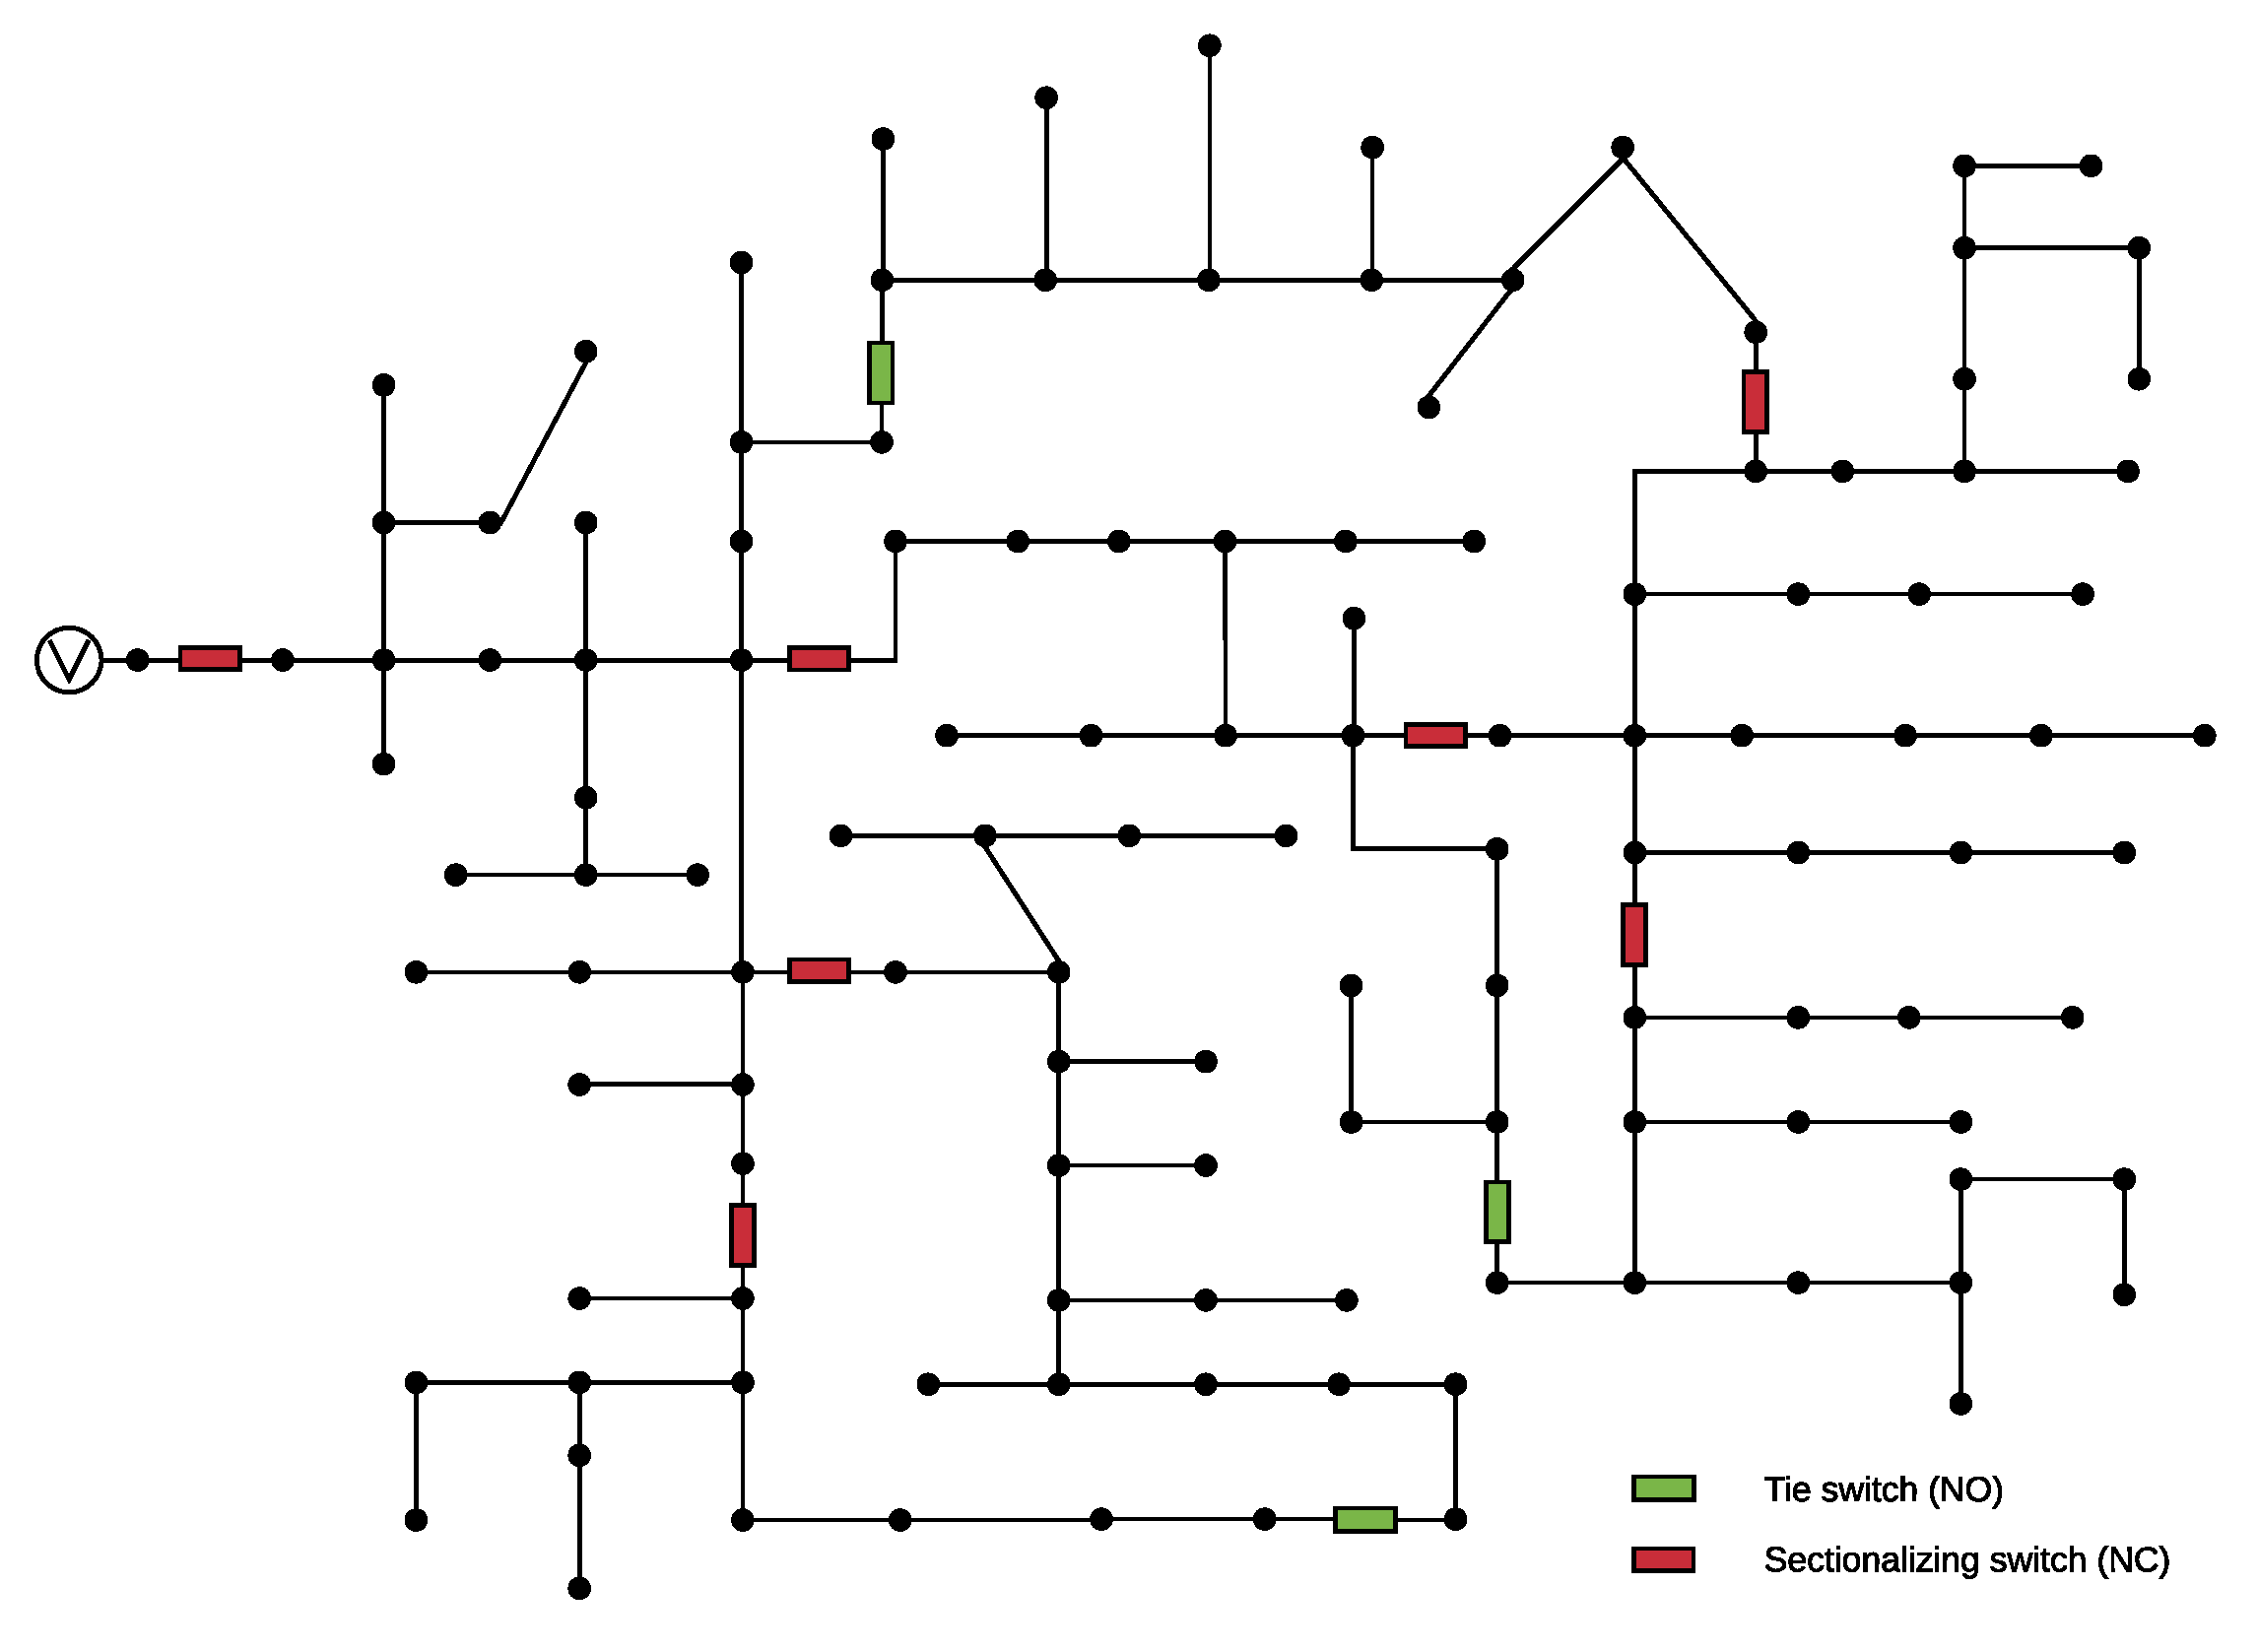
\includegraphics[scale=0.35]{_chapter2/fig/123iee_tc.pdf}
    \caption{IEEE 123 Node Test Feeder}
    \label{ch2:fig:123bus}
\end{figure}

%\subsection{IEEE 8500 Node Test Feeder}
%Figure \ref{ch2:fig:8500bus} shows the IEEE 123 node test feeder topology and Table \ref{ch2:tab:dn_data} summaries its
%parameters. This system is modified by reducing the number of switches to 25, due to computational capacities. 

%\begin{figure}
    \centering
    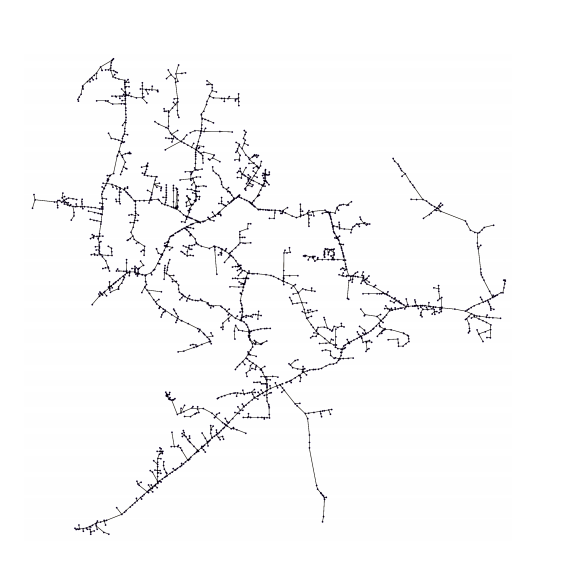
\includegraphics[scale=0.5]{_chapter2/fig/ieee8500.png}
    \caption{IEEE 8500 Node Test Feeder}
    \label{ch2:fig:8500bus}
\end{figure}


  \chapter{Service Restoration Algorithm Results}
\label{ch3}
This chapter presents the results of the Service Restoration algorithm proposed in this study 
for the IEEE test feeders described in the previous Chapter. 
Firstly, it presents RL parameters obtained from Training scenario. And then, it presents the 
Service Restoration plans as results of Production scenario. 

\section{RL Training Results}
The Service Restoration algorithm obtains the restoration plan through reinforcement learning training, 
as achieved in Chapter \ref{ch1}. Training scenario turns the network parameters into a Markov 
Decision Process, which defines the behavior and size of the algorithm operations.
Therefore, the numbers of lines and switches of the two test cases presented in Table \ref{ch2:tab:dn_data} are 
directly related to the number of states $n(S)$ and actions $n(A)$ presented in the following tables.

Additionally, Tables \ref{ch3:tab:td33}, \ref{ch3:tab:td123_1}, and \ref{ch3:tab:td123_2} show the 
elapsed time $T[min]$, the number of failures restored $n(FR)$, and the restoration rate $RR$ for each 
training relying on switch configurations in the IEEE 33 and the IEEE 123 Node Test Feeder.

\begin{table}
    \centering
    \caption{IEEE 33 - Training parameters 2sw - 5sw}
    \label{ch3:tab:td33}
    \begin{tabular}{lcccc} 
    \hline
    \multicolumn{1}{c}{\multirow{2}{*}{ \textbf{Data} }} & \multicolumn{4}{l}{\textbf{IEEE 33 Node Test Feeder}~ ~ }      \\ 
    \cline{2-5}
    \multicolumn{1}{c}{}                                 & \textbf{2sw}  & \textbf{3sw}  & \textbf{4sw}  & \textbf{5sw}   \\ 
    \hline
     \textbf{n(S)}                                       & 128           & 256           & 512           & 1024           \\
    \textbf{n(A)}                                        & 12            & 13            & 14            & 15             \\
    \textbf{T [min]}                                       & 1.3           & 2.9           & 5.6           & 10             \\
    \textbf{n(FR)}                                       & 20            & 28            & 31            & 31             \\
    \textbf{RR}                                          & 1             & 1             & 1             & 1              \\
    \hline
    \end{tabular}
    \end{table}
\begin{table}
    \centering
    \caption{IEEE 123 - Training parameters 5sw - 10sw}
    \label{ch3:tab:td123_1}
    \begin{tabular}{lcccccc} 
    \hline
    \multicolumn{1}{c}{\multirow{2}{*}{ \textbf{Data} }} & \multicolumn{6}{c}{\textbf{IEEE 123 Node Test Feeder} }                                         \\ 
    \cline{2-7}
    \multicolumn{1}{c}{}                                 & \textbf{5sw}  & \textbf{6sw}  & \textbf{7sw}  & \textbf{8sw}  & \textbf{9sw}  & \textbf{10sw}   \\ 
    \hline
     \textbf{n(S)}                                       & 3.744         & 7.588         & 14.976        & 29.952        & 59.904        & 119.808         \\
    \textbf{n(A)}                                        & 5             & 6             & 7             & 8             & 9             & 10              \\
    \textbf{T [min]}                                       & 7.3           & 8.4           & 11.0          & 15.5          & 17.7          & 41.3            \\
    \textbf{n(FR)}                                       & 0             & 0             & 14            & 22            & 22            & 41              \\
    \textbf{RR}                                          & 0             & 0             & 1             & 1             & 1             & 1               \\
    \hline
    \end{tabular}
    \end{table}
\begin{table}
    \centering
    \caption{IEEE 123 - Training parameters 11sw - 15sw}
    \label{ch3:tab:td123_2}
    \begin{tabular}{lccccc} 
    \hline
    \multicolumn{1}{c}{\multirow{2}{*}{ \textbf{Data} }} & \multicolumn{5}{c}{\textbf{IEEE 123 Node Test Feeder}~ ~ ~ ~~ }                     \\ 
    \cline{2-6}
    \multicolumn{1}{c}{}                                 & \textbf{11sw}  & \textbf{12sw}  & \textbf{13sw}  & \textbf{14sw}  & \textbf{15sw}   \\ 
    \hline
     \textbf{n(S)}                                       & 239.616        & 479.232        & 958.464        & 1.916.928      & 3.833.856       \\
    \textbf{n(A)}                                        & 11             & 12             & 13             & 14             & 15              \\
    \textbf{T [min]}                                       & 72.5           & 145.0          & 290.3          & 602.4          & 1198.2          \\
    \textbf{n(FR)}                                       &     43           &     45           &    45            &  46              &   51              \\
    \textbf{RR}                                          & 1              & 1              & 1              & 1              & 1               \\
    \hline
    \end{tabular}
    \end{table}

\section{Service Restoration Plans}

The Service Restoration Plan specifies the optimal switching operations to restore the maximum number of loads
maintaining the operational and topological constraints after a fault occurs. 
The execution of this plan is carried out in the Production scenario, that is, once the system is already trained.

Tables \ref{ch2:tab:33_actions} and \ref{ch2:tab:123_actions} present the restoration plans for IEEE 33 Node Test Feeder with 5 switches 
and IEEE 123 Node Test Feeder with 10 switches, respectively. Additionally, they contain the number of actions required $n(A)$, 
the processing time (T[s]), the number of isolated loads before $n(IL)_{pre}$ and after $n(IL)_{post}$  restoration, and the restoration rate ($RR$).
The latter is calculated as follows: $ RR = \frac{n(IL)_{prev}-n(IL)_{post}}{n(IL)_{prev}}$.

The Service Restoration Plans for the other switch configurations of the test cases are presented in Appendix \ref{appx-a:additional-results}.
\begin{table}
    \centering
    \caption{SR plan - IEEE 33 Node Test Feeder - 5 switches}
    \label{ch2:tab:33_actions}
    \begin{tabular}{llccccc}
    \hline
    \textbf{\begin{tabular}[c]{@{}l@{}}Faulted\\  line\end{tabular}} & \textbf{Actions}    & \textbf{N(A)} & \textbf{T {[}s{]}} & \textbf{N(IL)$_{pre}$} & \textbf{N(IL)$_{post}$} & \textbf{RR} \\ \hline
    \textit{\textbf{l1}}                                             & {[}('s33', None){]} & 0             & 0.005               & 32             & 32             & 0           \\
    \textit{\textbf{l2}}                                             & {[}('s35', 1){]}    & 1             & 0.005               & 26             & 0              & 1           \\
    \textit{\textbf{l3}}                                             & {[}('s37', 1){]}    & 1             & 0.005              & 22             & 0              & 1           \\
    \textit{\textbf{l4}}                                             & {[}('s37', 1){]}    & 1             & 0.005               & 21             & 0              & 1           \\
    \textit{\textbf{l5}}                                             & {[}('s37', 1){]}    & 1             & 0.005               & 20             & 0              & 1           \\
    \textit{\textbf{l6}}                                             & {[}('s36', 1){]}    & 1             & 0.005               & 12             & 0              & 1           \\
    \textit{\textbf{l7}}                                             & {[}('s36', 1){]}    & 1             & 0.004               & 11             & 0              & 1           \\
    \textit{\textbf{l8}}                                             & {[}('s36', 1){]}    & 1             & 0.005               & 10             & 0              & 1           \\
    \textit{\textbf{l9}}                                             & {[}('s36', 1){]}    & 1             & 0.004               & 9              & 0              & 1           \\
    \textit{\textbf{l10}}                                            & {[}('s36', 1){]}    & 1             & 0.004               & 8              & 0              & 1           \\
    \textit{\textbf{l11}}                                            & {[}('s36', 1){]}    & 1             & 0.005               & 7              & 0              & 1           \\
    \textit{\textbf{l12}}                                            & {[}('s36', 1){]}    & 1             & 0.005               & 6              & 0              & 1           \\
    \textit{\textbf{l13}}                                            & {[}('s36', 1){]}    & 1             & 0.004               & 5              & 0              & 1           \\
    \textit{\textbf{l14}}                                            & {[}('s36', 1){]}    & 1             & 0.005               & 4              & 0              & 1           \\
    \textit{\textbf{l15}}                                            & {[}('s36', 1){]}    & 1             & 0.005               & 3              & 0              & 1           \\
    \textit{\textbf{l16}}                                            & {[}('s36', 1){]}    & 1             & 0.004               & 2              & 0              & 1           \\
    \textit{\textbf{l17}}                                            & {[}('s36', 1){]}    & 1             & 0.004               & 1              & 0              & 1           \\
    \textit{\textbf{l18}}                                            & {[}('s35', 1){]}    & 1             & 0.005               & 5              & 0              & 1           \\
    \textit{\textbf{l19}}                                            & {[}('s35', 1){]}    & 1             & 0.005               & 4              & 0              & 1           \\
    \textit{\textbf{l20}}                                            & {[}('s35', 1){]}    & 1             & 0.005               & 2              & 0              & 1           \\
    \textit{\textbf{l21}}                                            & {[}('s35', 1){]}    & 1             & 0.005               & 1              & 0              & 1           \\
    \textit{\textbf{l22}}                                            & {[}('s37', 1){]}    & 1             & 0.005               & 3              & 0              & 1           \\
    \textit{\textbf{l23}}                                            & {[}('s37', 1){]}    & 1             & 0.005               & 2              & 0              & 1           \\
    \textit{\textbf{l24}}                                            & {[}('s37', 1){]}    & 1             & 0.005               & 1              & 0              & 1           \\
    \textit{\textbf{l25}}                                            & {[}('s37', 1){]}    & 1             & 0.004               & 7              & 0              & 1           \\
    \textit{\textbf{l26}}                                            & {[}('s37', 1){]}    & 1             & 0.005               & 6              & 0              & 1           \\
    \textit{\textbf{l27}}                                            & {[}('s37', 1){]}    & 1             & 0.005               & 5              & 0              & 1           \\
    \textit{\textbf{l28}}                                            & {[}('s37', 1){]}    & 1             & 0.005               & 4              & 0              & 1           \\
    \textit{\textbf{l29}}                                            & {[}('s36', 1){]}    & 1             & 0.005               & 3              & 0              & 1           \\
    \textit{\textbf{l30}}                                            & {[}('s36', 1){]}    & 1             & 0.005               & 3              & 0              & 1           \\
    \textit{\textbf{l31}}                                            & {[}('s36', 1){]}    & 1             & 0.005               & 2              & 0              & 1           \\
    \textit{\textbf{l32}}                                            & {[}('s36', 1){]}    & 1             & 0.004               & 1              & 0              & 1           \\ \hline
    \end{tabular}
    \end{table}
\begin{table}
    \centering
    \caption{SR plan - IEEE 123 Node Test Feeder - 10 switches }
    \label{ch2:tab:123_actions}
    \begin{tabular}{llccccc}
    \hline
    \textbf{\begin{tabular}[c]{@{}l@{}}Faulted\\  line\end{tabular}} & \textbf{Actions}             & \textbf{N(A)} & \textbf{T {[}s{]}} & \textbf{N(IL)$_{pre}$} & \textbf{N(IL)$_{post}$} & \textbf{RR} \\ \hline
    \textit{\textbf{l116}}                                           & {[}('sw7', 1){]}             & 1             & 0.016              & 52             & 0              & 1           \\
    \textit{\textbf{l52}}                                            & {[}('sw7', 1){]}             & 1             & 0.016              & 51             & 0              & 1           \\
    \textit{\textbf{l53}}                                            & {[}('sw7', 1){]}             & 1             & 0.017              & 50             & 0              & 1           \\
    \textit{\textbf{l55}}                                            & {[}('sw7', 1){]}             & 1             & 0.016              & 48             & 0              & 1           \\
    \textit{\textbf{l58}}                                            & {[}('sw7', 1){]}             & 1             & 0.018              & 46             & 0              & 1           \\
    \textit{\textbf{l117}}                                           & {[}('sw7', 1){]}             & 1             & 0.016              & 38             & 0              & 1           \\
    \textit{\textbf{l67}}                                            & {[}('sw7', 1){]}             & 1             & 0.017              & 21             & 0              & 1           \\
    \textit{\textbf{l73}}                                            & {[}('sw7', 1){]}             & 1             & 0.016              & 18             & 0              & 1           \\
    \textit{\textbf{l77}}                                            & {[}('sw7', 1){]}             & 1             & 0.017              & 8              & 0              & 1           \\
    \textit{\textbf{l86}}                                            & {[}('sw7', 1){]}             & 1             & 0.016              & 7              & 0              & 1           \\
    \textit{\textbf{l88}}                                            & {[}('sw7', 1){]}             & 1             & 0.017              & 5              & 0              & 1           \\
    \textit{\textbf{l90}}                                            & {[}('sw7', 1){]}             & 1             & 0.016              & 4              & 0              & 1           \\
    \textit{\textbf{l92}}                                            & {[}('sw7', 1){]}             & 1             & 0.017              & 3              & 0              & 1           \\
    \textit{\textbf{l94}}                                            & {[}('sw7', 1){]}             & 1             & 0.016              & 2              & 0              & 1           \\
    \textit{\textbf{l17}}                                            & {[}('sw7', 1){]}             & 1             & 0.017              & 1              & 0              & 1           \\
    \textit{\textbf{l34}}                                            & {[}('sw7', 1){]}             & 1             & 0.018              & 2              & 0              & 1           \\
    \textit{\textbf{l68}}                                            & {[}('sw10', 1){]}            & 1             & 0.016              & 13             & 0              & 1           \\
    \textit{\textbf{l118}}                                           & {[}('sw10', 1){]}            & 1             & 0.016              & 10             & 0              & 1           \\
    \textit{\textbf{l101}}                                           & {[}('sw10', 1){]}            & 1             & 0.016              & 7              & 0              & 1           \\
    \textit{\textbf{l105}}                                           & {[}('sw10', 1){]}            & 1             & 0.016              & 5              & 0              & 1           \\
    \textit{\textbf{l63}}                                            & {[}('sw10', 1){]}            & 1             & 0.017              & 5              & 0              & 1           \\
    \textit{\textbf{l62}}                                            & {[}('sw10', 1){]}            & 1             & 0.016              & 6              & 0              & 1           \\
    \textit{\textbf{l61}}                                            & {[}('sw10', 1){]}            & 1             & 0.017              & 7              & 0              & 1           \\
    \textit{\textbf{l114}}                                           & {[}('sw9', 1){]}             & 1             & 0.017              & 16             & 0              & 1           \\
    \textit{\textbf{l36}}                                            & {[}('sw9', 1){]}             & 1             & 0.016              & 12             & 0              & 1           \\
    \textit{\textbf{l41}}                                            & {[}('sw9', 1){]}             & 1             & 0.016              & 11             & 0              & 1           \\
    \textit{\textbf{l43}}                                            & {[}('sw9', 1){]}             & 1             & 0.018              & 9              & 0              & 1           \\
    \textit{\textbf{l45}}                                            & {[}('sw9', 1){]}             & 1             & 0.017              & 7              & 0              & 1           \\
    \textit{\textbf{l48}}                                            & {[}('sw9', 1){]}             & 1             & 0.016              & 5              & 0              & 1           \\
    \textit{\textbf{l49}}                                            & {[}('sw9', 1){]}             & 1             & 0.020              & 2              & 0              & 1           \\
    \textit{\textbf{l50}}                                            & {[}('sw9', 1){]}             & 1             & 0.017              & 1              & 0              & 1           \\
    \textit{\textbf{l31}}                                            & {[}('sw9', 1){]}             & 1             & 0.017              & 1              & 0              & 1           \\
    \textit{\textbf{l30}}                                            & {[}('sw9', 1){]}             & 1             & 0.017              & 2              & 0              & 1           \\
    \textit{\textbf{l26}}                                            & {[}('sw9', 1){]}             & 1             & 0.017              & 3              & 0              & 1           \\
    \textit{\textbf{l24}}                                            & {[}('sw9', 1){]}             & 1             & 0.017              & 6              & 0              & 1           \\
    \textit{\textbf{l22}}                                            & {[}('sw9', 1), ('sw6', 0){]} & 2             & 0.018              & 7              & 0              & 1           \\
    \textit{\textbf{l19}}                                            & {[}('sw9', 1){]}             & 1             & 0.017              & 8              & 0              & 1           \\
    \textit{\textbf{l12}}                                            & {[}('sw7', 1){]}             & 1             & 0.018              & 3              & 0              & 1           \\
    \textit{\textbf{l115}}                                           & {[}('sw5', None){]}          & 0             & 0.017              & 91             & 91             & 0           \\
    \textit{\textbf{l5}}                                             & {[}('sw7', None){]}          & 0             & 0.016              & 2              & 2              & 0           \\
    \textit{\textbf{l1}}                                             & {[}('sw3', None){]}          & 0             & 0.016              & 1              & 1              & 0           \\ \hline
    \end{tabular}
    \end{table}

  \chapter{Discussion and Conclusion}
\label{ch-conclusions}

%\section{Future work}
\label{ch-conclusions:sec:future-work}
\section{Results Discussions}

The results obtained in the previous Chapter show that Service Restoration depends on the availability 
of transferring out-of-service un-faulted loads to healthy feeders, which in turn depends on the number 
and location of switches, i.e., if the location and number of switches are conducive, the SR algorithm 
can resupply all out-of-service un-faulted loads. 

Therefore, the SR algorithm obtained the optimal switch operations sequence for failure scenarios in 
which there was the possibility of transferring isolated loads to healthy feeders, and for those 
scenarios it restored all loads. 

The optimal sequence is obtained in the Training scenario but constantly updated in the Production
scenario. Consequently, the RL algorithm requires retraining when system variations occur that increase or 
reduce the numbers of lines or switches, but retraining is not required when these changes affect the 
number of loads. 

\subsection{SR Algorithm performance}
The performance of this algorithm relies on computational capacity: memory size and processing.

First, the RL model dictates the memory size required. This is because of the model needs to compute a Q 
Values matrix, whose size depends on the numbers of actions and states and, in turn, on the numbers of 
lines and switches, as explained in Chapter 3. Accordingly, Figure \ref{ch-conclusions:fig:memory} shows the amount of 
memory needed under the numbers of lines and switches for the IEEE 123 Node Test Feeder with 10 switches.
As a result, memory size grows linearly with an increase in the number of lines and exponentially with 
an increase in the number of switches. 
\begin{figure}[!ht]
    \centering
	\subfloat[Memory size according to number of switches ]{
        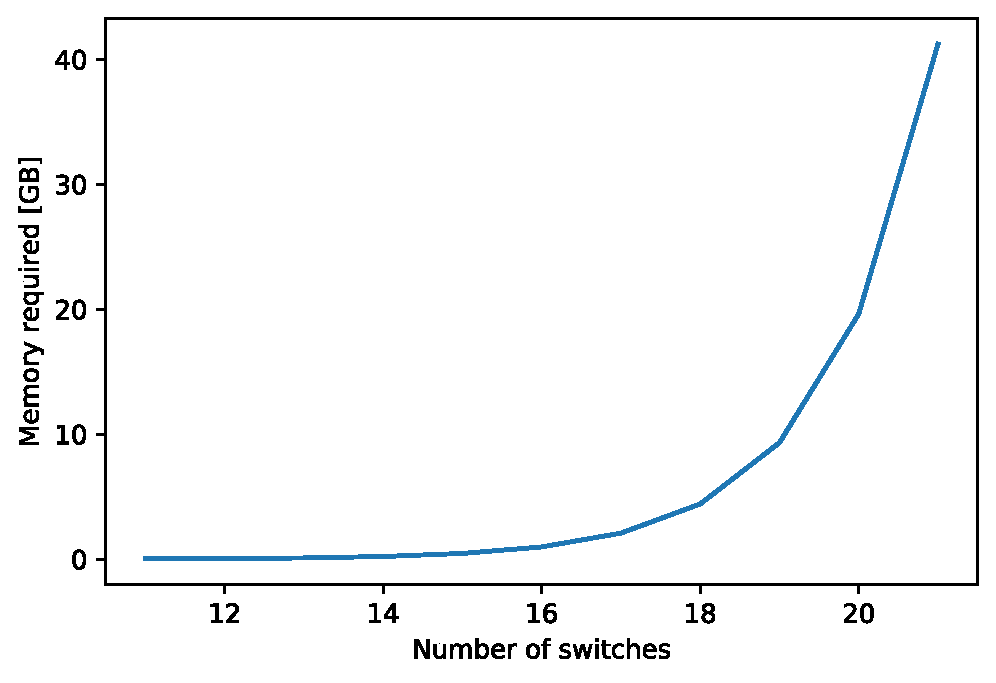
\includegraphics[scale=0.4]{_conclusions/fig/switches.pdf}
		\label{ch-conclusions:fig:ms_switches}
	}%
	\qquad
	\subfloat[Memory size according to number of lines]{
        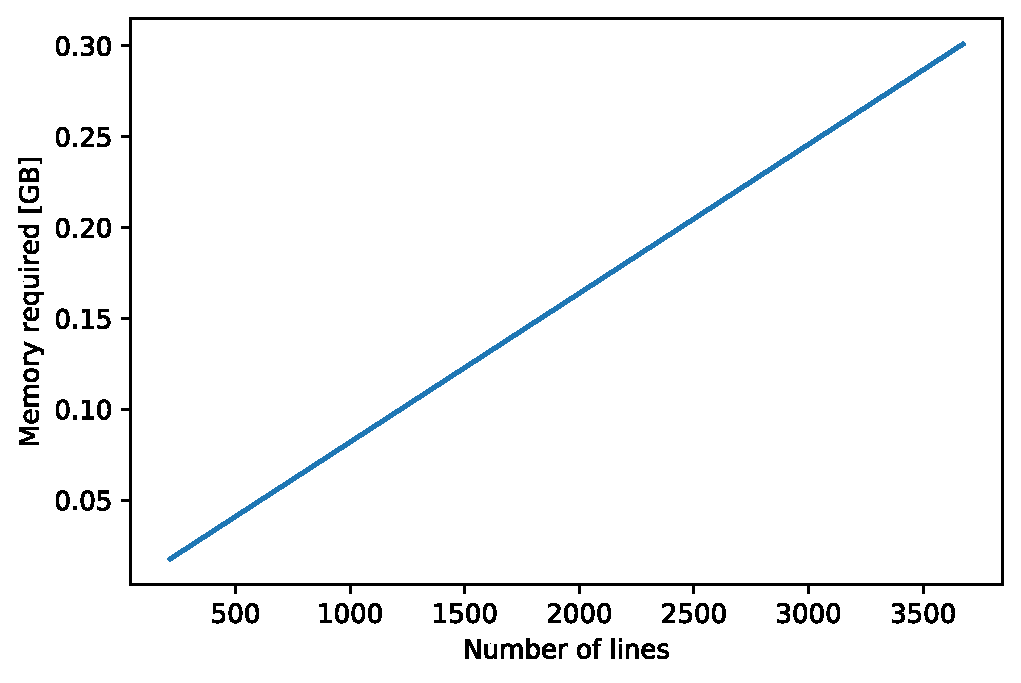
\includegraphics[scale=0.4]{_conclusions/fig/lines.pdf}
		\label{ch-conclusions:fig:ms_lines}
	}
	\caption{Memory size comparison according to numbers of lines and switches variations for the IEEE 123 Node Test Feeder - 10 switches}
	\label{ch-conclusions:fig:memory}	
\end{figure}


Since the number of switches is the factor that most affects the size of the model, Figure \ref{ch-conclusions:fig:123_swtimestates} 
presents the required processing time and the number of states according to the number of switches for the IEEE 123 Node Test Feeder.


\begin{figure}
    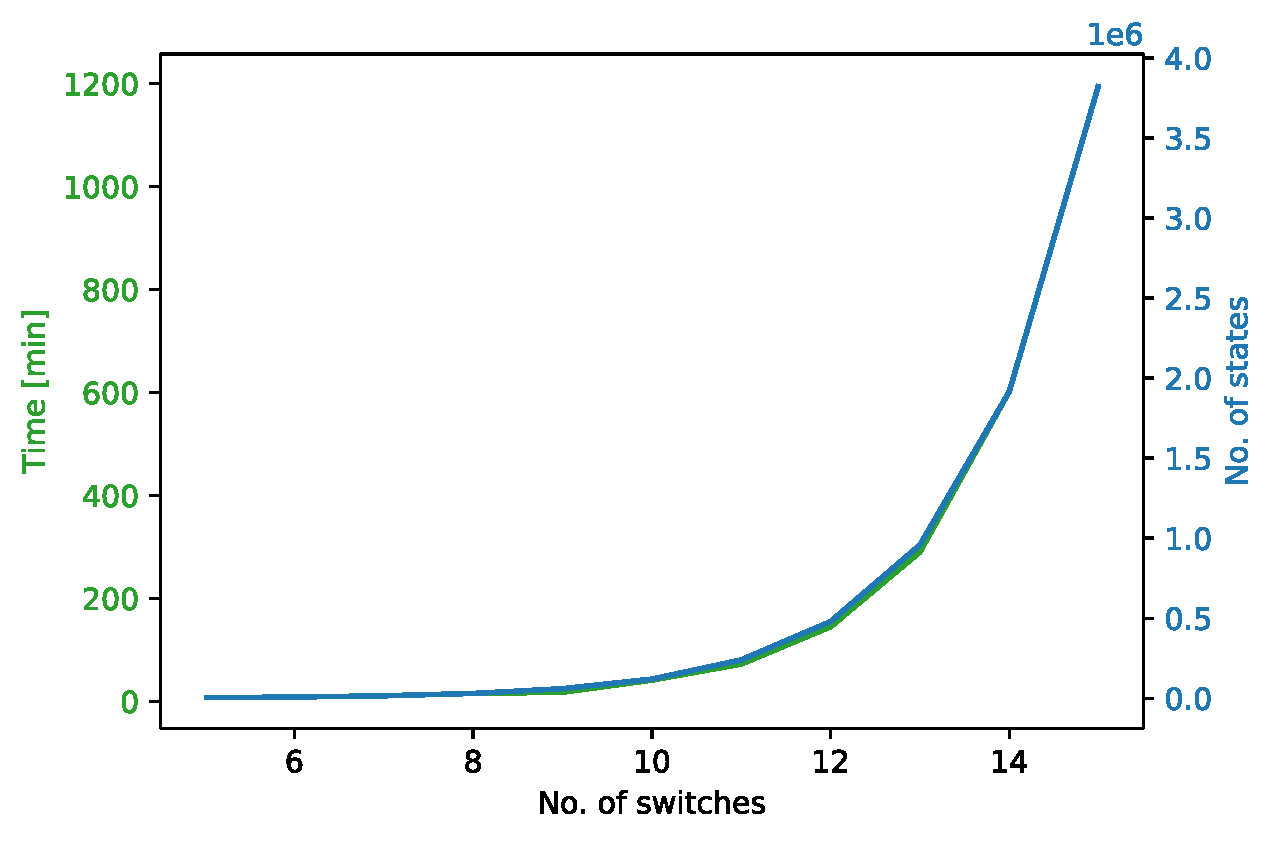
\includegraphics[scale=0.5]{_conclusions/fig/swtimestates.pdf}
    \centering
    \caption{No. of switches vs Time [min] and No. of states - IEEE 123 Node Test Feeder}
    \label{ch-conclusions:fig:123_swtimestates}
\end{figure}
\newpage 
\newpage

\section{Conclusion}
\label{ch-conclusions:sec:conclusion}


This thesis aimed to present the development of a Service Restoration Algorithm implementing Reinforcement Learning techniques.

The reviewed literature in Chapter 2 emphasized the need for improving Service Restoration methodologies by developing new approaches that endow Distribution Networks with a self-healing capacity to resupply automatically and intelligently out-of-service un-faulted customers after a fault occurrence.  

Chapter 3 explains the Reinforcement Learning technique implemented throughout modeling a Markov Decision Process that captures the Distribution Network parameters, the multiobjective optimization function, and the operational and topological constraints. Furthermore, it states the roles of the co-simulation engine and how it is integrated into the algorithm. As a result, Chapter 3 proposes an algorithm structure that divides the Service Restoration algorithm into Training and Production scenarios, both implementing an RL technique and a co-simulation engine.  

Lastly, Chapter 4 defines the SR algorithm validation including test cases and results. The test cases compromise both IEEE 33 bus test feeder and IEEE 123 bus test feeder. In this way, the Service Restoration algorithm was tested for each of the test cases, thus obtaining a restoration plan for a fault under each of its lines. 

The service restoration plan obtained for the IEEE 33 Node Test Feeder and the IEEE 123 Node Test Feeder successfully resupply $100\%$ of the out-of-service un-faulted customers, as described by the restoration rate presented in Tables \ref{ch2:tab:33_actions} and \ref{ch2:tab:123_actions}.

%The SR algorithm built upon the outlined limitations in the literature 

In conclusion, this SR algorithm proposed is capable of self-learning to obtain an optimal solution that fulfills operational and topological constraints. Furthermore, it establishes a new approach in service restoration methodologies by implementing a Reinforcement Learning technique.

  % next line adds the Bibliography to the contents page
  \addcontentsline{toc}{chapter}{References}
  % uncomment next line to change bibliography name to references
  \renewcommand{\bibname}{References}
  \bibliography{references}
  \bibliographystyle{ieeetr}  %use the plain bibliography style


  % now enable appendix numbering format and include any appendices
  \appendix
  \chapter{Additional Results}
\label{appx-a:additional-results}


\section{Service Resotoration Plans}

\begin{table}
    \centering
    \caption{SR plan for IEEE 123 Node Test Feeder with 7 switches}
    \label{app:tab:123_7sw}
    \begin{tabular}{llccccc} 
    \hline
    \multicolumn{1}{c}{\begin{tabular}[c]{@{}c@{}}\textbf{Faulted }\\\textbf{line}\end{tabular}} & \multicolumn{1}{c}{\textbf{Actions}} & \textbf{n(A)} & \textbf{T [s]} & \textbf{n(IL)$_{pre}$} & \textbf{n(IL)$_{post}$} & \multicolumn{1}{c|}{\textbf{RR}}  \\ 
    \hline
    \textbf{\textit{l19}}                                                                        & {[}('sw9', 1)]                       & 1             & 0.015          & 8              & 0              & 1                                 \\
    \textbf{\textit{l22}}                                                                        & {[}('sw9', 1)]                       & 1             & 0.016          & 7              & 0              & 1                                 \\
    \textbf{\textit{l24}}                                                                        & {[}('sw9', 1)]                       & 1             & 0.016          & 6              & 0              & 1                                 \\
    \textbf{\textit{l26}}                                                                        & {[}('sw9', 1)]                       & 1             & 0.015          & 3              & 0              & 1                                 \\
    \textbf{\textit{l30}}                                                                        & {[}('sw9', 1)]                       & 1             & 0.017          & 2              & 0              & 1                                 \\
    \textbf{\textit{l31}}                                                                        & {[}('sw9', 1)]                       & 1             & 0.016          & 1              & 0              & 1                                 \\
    \textbf{\textit{l50}}                                                                        & {[}('sw9', 1)]                       & 1             & 0.017          & 1              & 0              & 1                                 \\
    \textbf{\textit{l49}}                                                                        & {[}('sw9', 1)]                       & 1             & 0.018          & 2              & 0              & 1                                 \\
    \textbf{\textit{l48}}                                                                        & {[}('sw9', 1)]                       & 1             & 0.016          & 5              & 0              & 1                                 \\
    \textbf{\textit{l45}}                                                                        & {[}('sw9', 1)]                       & 1             & 0.016          & 7              & 0              & 1                                 \\
    \textbf{\textit{l43}}                                                                        & {[}('sw9', 1)]                       & 1             & 0.016          & 9              & 0              & 1                                 \\
    \textbf{\textit{l41}}                                                                        & {[}('sw9', 1)]                       & 1             & 0.017          & 11             & 0              & 1                                 \\
    \textbf{\textit{l36}}                                                                        & {[}('sw9', 1)]                       & 1             & 0.017          & 12             & 0              & 1                                 \\
    \textbf{\textit{l114}}                                                                       & {[}('sw9', 1)]                       & 1             & 0.017          & 16             & 0              & 1                                 \\
    \hline
    \end{tabular}
    \end{table}
\begin{table}
    \centering
    \caption{SR plan for IEEE 123 Node Test Feeder with 8 switches}
    \label{app:tab:123_8sw}
    \begin{tabular}{llccccc}
    \hline
    \textbf{\begin{tabular}[c]{@{}l@{}}Faulted\\ line\end{tabular}} & \textbf{Actions}  & \textbf{n(A)} & \textbf{T {[}s{]}} & \textbf{n(IL)$_{pre}$} & \textbf{n(IL)$_{post}$} & \textbf{RR} \\ \hline
    \textit{\textbf{l117}}                                          & {[}('sw10', 1){]} & 1             & 0.015              & 38             & 0              & 1           \\
    \textit{\textbf{l68}}                                           & {[}('sw10', 1){]} & 1             & 0.016              & 13             & 0              & 1           \\
    \textit{\textbf{l118}}                                          & {[}('sw10', 1){]} & 1             & 0.016              & 10             & 0              & 1           \\
    \textit{\textbf{l101}}                                          & {[}('sw10', 1){]} & 1             & 0.016              & 7              & 0              & 1           \\
    \textit{\textbf{l105}}                                          & {[}('sw10', 1){]} & 1             & 0.016              & 5              & 0              & 1           \\
    \textit{\textbf{l63}}                                           & {[}('sw10', 1){]} & 1             & 0.016              & 5              & 0              & 1           \\
    \textit{\textbf{l62}}                                           & {[}('sw10', 1){]} & 1             & 0.016              & 6              & 0              & 1           \\
    \textit{\textbf{l61}}                                           & {[}('sw10', 1){]} & 1             & 0.017              & 7              & 0              & 1           \\
    \textit{\textbf{l114}}                                          & {[}('sw9', 1){]}  & 1             & 0.015              & 16             & 0              & 1           \\
    \textit{\textbf{l36}}                                           & {[}('sw9', 1){]}  & 1             & 0.016              & 12             & 0              & 1           \\
    \textit{\textbf{l41}}                                           & {[}('sw9', 1){]}  & 1             & 0.017              & 11             & 0              & 1           \\
    \textit{\textbf{l43}}                                           & {[}('sw9', 1){]}  & 1             & 0.017              & 9              & 0              & 1           \\
    \textit{\textbf{l45}}                                           & {[}('sw9', 1){]}  & 1             & 0.017              & 7              & 0              & 1           \\
    \textit{\textbf{l48}}                                           & {[}('sw9', 1){]}  & 1             & 0.016              & 5              & 0              & 1           \\
    \textit{\textbf{l49}}                                           & {[}('sw9', 1){]}  & 1             & 0.017              & 2              & 0              & 1           \\
    \textit{\textbf{l50}}                                           & {[}('sw9', 1){]}  & 1             & 0.017              & 1              & 0              & 1           \\
    \textit{\textbf{l31}}                                           & {[}('sw9', 1){]}  & 1             & 0.016              & 1              & 0              & 1           \\
    \textit{\textbf{l30}}                                           & {[}('sw9', 1){]}  & 1             & 0.016              & 2              & 0              & 1           \\
    \textit{\textbf{l26}}                                           & {[}('sw9', 1){]}  & 1             & 0.018              & 3              & 0              & 1           \\
    \textit{\textbf{l24}}                                           & {[}('sw9', 1){]}  & 1             & 0.016              & 6              & 0              & 1           \\
    \textit{\textbf{l22}}                                           & {[}('sw9', 1){]}  & 1             & 0.016              & 7              & 0              & 1           \\
    \textit{\textbf{l19}}                                           & {[}('sw9', 1){]}  & 1             & 0.016              & 8              & 0              & 1           \\ \hline
    \end{tabular}
    \end{table}
\begin{table}
    \centering
    \caption{SR plan for IEEE 123 Node Test Feeder with 9 switches}
    \label{app:tab:123_9sw}
    \begin{tabular}{lllllll}
    \hline
    \textbf{\begin{tabular}[c]{@{}l@{}}Faulted\\ line\end{tabular}} & \textbf{Actions}  & \multicolumn{1}{c}{\textbf{n(A)}} & \multicolumn{1}{c}{\textbf{T {[}s{]}}} & \multicolumn{1}{c}{\textbf{n(IL)$_{pre}$}} & \multicolumn{1}{c}{\textbf{n(IL)$_{post}$}} & \multicolumn{1}{c}{\textbf{RR}} \\ \hline
    \textit{\textbf{l68}}                                           & {[}('sw10', 1){]} & 1                                 & 0.017                                  & 13                                 & 0                                  & 13                              \\
    \textit{\textbf{l118}}                                          & {[}('sw10', 1){]} & 1                                 & 0.018                                  & 10                                 & 0                                  & 10                              \\
    \textit{\textbf{l101}}                                          & {[}('sw10', 1){]} & 1                                 & 0.016                                  & 7                                  & 0                                  & 7                               \\
    \textit{\textbf{l105}}                                          & {[}('sw10', 1){]} & 1                                 & 0.016                                  & 5                                  & 0                                  & 5                               \\
    \textit{\textbf{l63}}                                           & {[}('sw10', 1){]} & 1                                 & 0.016                                  & 5                                  & 0                                  & 5                               \\
    \textit{\textbf{l62}}                                           & {[}('sw10', 1){]} & 1                                 & 0.017                                  & 6                                  & 0                                  & 6                               \\
    \textit{\textbf{l61}}                                           & {[}('sw10', 1){]} & 1                                 & 0.017                                  & 7                                  & 0                                  & 7                               \\
    \textit{\textbf{l117}}                                          & {[}('sw10', 1){]} & 1                                 & 0.016                                  & 38                                 & 0                                  & 38                              \\
    \textit{\textbf{l19}}                                           & {[}('sw9', 1){]}  & 1                                 & 0.016                                  & 8                                  & 0                                  & 8                               \\
    \textit{\textbf{l22}}                                           & {[}('sw9', 1){]}  & 1                                 & 0.015                                  & 7                                  & 0                                  & 7                               \\
    \textit{\textbf{l24}}                                           & {[}('sw9', 1){]}  & 1                                 & 0.016                                  & 6                                  & 0                                  & 6                               \\
    \textit{\textbf{l26}}                                           & {[}('sw9', 1){]}  & 1                                 & 0.016                                  & 3                                  & 0                                  & 3                               \\
    \textit{\textbf{l30}}                                           & {[}('sw9', 1){]}  & 1                                 & 0.017                                  & 2                                  & 0                                  & 2                               \\
    \textit{\textbf{l31}}                                           & {[}('sw9', 1){]}  & 1                                 & 0.015                                  & 1                                  & 0                                  & 1                               \\
    \textit{\textbf{l50}}                                           & {[}('sw9', 1){]}  & 1                                 & 0.016                                  & 1                                  & 0                                  & 1                               \\
    \textit{\textbf{l49}}                                           & {[}('sw9', 1){]}  & 1                                 & 0.017                                  & 2                                  & 0                                  & 2                               \\
    \textit{\textbf{l48}}                                           & {[}('sw9', 1){]}  & 1                                 & 0.017                                  & 5                                  & 0                                  & 5                               \\
    \textit{\textbf{l45}}                                           & {[}('sw9', 1){]}  & 1                                 & 0.017                                  & 7                                  & 0                                  & 7                               \\
    \textit{\textbf{l43}}                                           & {[}('sw9', 1){]}  & 1                                 & 0.016                                  & 9                                  & 0                                  & 9                               \\
    \textit{\textbf{l41}}                                           & {[}('sw9', 1){]}  & 1                                 & 0.017                                  & 11                                 & 0                                  & 11                              \\
    \textit{\textbf{l36}}                                           & {[}('sw9', 1){]}  & 1                                 & 0.016                                  & 12                                 & 0                                  & 12                              \\
    \textit{\textbf{l114}}                                          & {[}('sw9', 1){]}  & 1                                 & 0.015                                  & 16                                 & 0                                  & 16                              \\ \hline
    \end{tabular}
    \end{table}
\begin{table}
    \centering
    \caption{SR plan for IEEE 123 Node Test Feeder with 15 switches - part 1}
    \label{ch-app-12315swp2}
    \begin{tabular}{llccccc}
    \hline
    \textbf{\begin{tabular}[c]{@{}l@{}}Faulted\\ line\end{tabular}} & \textbf{Actions}                          & \textbf{n(A)} & \textbf{T {[}s{]}} & \textbf{n(IL)} & \textbf{n(IL)} & \textbf{RR} \\ \hline
    \textit{\textbf{l2}}                                            & {[}('sw15', 1){]}                         & 1             & 0.018              & 3              & 0              & 1           \\
    \textit{\textbf{l5}}                                            & {[}('sw15', 1){]}                         & 1             & 0.017              & 2              & 0              & 1           \\
    \textit{\textbf{l6}}                                            & {[}('sw15', 1){]}                         & 1             & 0.018              & 1              & 0              & 1           \\
    \textit{\textbf{l3}}                                            & {[}('sw15', 1){]}                         & 1             & 0.016              & 86             & 0              & 1           \\
    \textit{\textbf{l7}}                                            & {[}('sw15', 1){]}                         & 1             & 0.016              & 85             & 0              & 1           \\
    \textit{\textbf{l9}}                                            & {[}('sw14', 1){]}                         & 1             & 0.017              & 3              & 0              & 1           \\
    \textit{\textbf{l11}}                                           & {[}('sw14', 1){]}                         & 1             & 0.018              & 2              & 0              & 1           \\
    \textit{\textbf{l14}}                                           & {[}('sw14', 1){]}                         & 1             & 0.016              & 1              & 0              & 1           \\
    \textit{\textbf{l20}}                                           & {[}('sw14', 1){]}                         & 1             & 0.017              & 1              & 0              & 1           \\
    \textit{\textbf{l18}}                                           & {[}('sw14', 1){]}                         & 1             & 0.017              & 2              & 0              & 1           \\
    \textit{\textbf{l13}}                                           & {[}('sw14', 1), ('sw3', 0), ('sw9', 1){]} & 3             & 0.019              & 26             & 9              & 0.7         \\
    \textit{\textbf{l12}}                                           & {[}('sw15', 1){]}                         & 1             & 0.022              & 3              & 0              & 1           \\
    \textit{\textbf{l34}}                                           & {[}('sw15', 1){]}                         & 1             & 0.018              & 2              & 0              & 1           \\
    \textit{\textbf{l17}}                                           & {[}('sw7', 1){]}                          & 1             & 0.017              & 1              & 0              & 1           \\
    \textit{\textbf{l90}}                                           & {[}('sw7', 1){]}                          & 1             & 0.017              & 4              & 0              & 1           \\
    \textit{\textbf{l88}}                                           & {[}('sw7', 1){]}                          & 1             & 0.017              & 5              & 0              & 1           \\
    \textit{\textbf{l86}}                                           & {[}('sw7', 1){]}                          & 1             & 0.017              & 7              & 0              & 1           \\
    \textit{\textbf{l77}}                                           & {[}('sw7', 1){]}                          & 1             & 0.018              & 8              & 0              & 1           \\
    \textit{\textbf{l73}}                                           & {[}('sw7', 1){]}                          & 1             & 0.017              & 18             & 0              & 1           \\
    \textit{\textbf{l67}}                                           & {[}('sw7', 1){]}                          & 1             & 0.017              & 21             & 0              & 1           \\
    \textit{\textbf{l68}}                                           & {[}('sw10', 1){]}                         & 1             & 0.016              & 13             & 0              & 1           \\
    \textit{\textbf{l118}}                                          & {[}('sw10', 1){]}                         & 1             & 0.017              & 10             & 0              & 1           \\
    \textit{\textbf{l101}}                                          & {[}('sw10', 1){]}                         & 1             & 0.016              & 7              & 0              & 1           \\
    \textit{\textbf{l105}}                                          & {[}('sw10', 1){]}                         & 1             & 0.017              & 5              & 0              & 1           \\
    \textit{\textbf{l63}}                                           & {[}('sw13', 1){]}                         & 1             & 0.017              & 5              & 0              & 1           \\
    \textit{\textbf{l62}}                                           & {[}('sw13', 1){]}                         & 1             & 0.018              & 6              & 0              & 1           \\
    \textit{\textbf{l61}}                                           & {[}('sw13', 1){]}                         & 1             & 0.017              & 7              & 0              & 1           \\
    \textit{\textbf{l58}}                                           & {[}('sw13', 1){]}                         & 1             & 0.022              & 46             & 0              & 1           \\
    \textit{\textbf{l55}}                                           & {[}('sw13', 1){]}                         & 1             & 0.017              & 48             & 0              & 1           \\
    \textit{\textbf{l53}}                                           & {[}('sw13', 1){]}                         & 1             & 0.016              & 50             & 0              & 1           \\
    \textit{\textbf{l52}}                                           & {[}('sw13', 1){]}                         & 1             & 0.017              & 51             & 0              & 1           \\
    \textit{\textbf{l116}}                                          & {[}('sw13', 1){]}                         & 1             & 0.017              & 52             & 0              & 1           \\
    \textit{\textbf{l64}}                                           & {[}('sw13', 1){]}                         & 1             & 0.016              & 4              & 0              & 1           \\
    \textit{\textbf{l65}}                                           & {[}('sw13', 1){]}                         & 1             & 0.017              & 1              & 0              & 1           \\
    \textit{\textbf{l40}}                                           & {[}('sw13', 1){]}                         & 1             & 0.017              & 1              & 0              & 1           \\
    \textit{\textbf{l41}}                                           & {[}('sw9', 1){]}                          & 1             & 0.016              & 11             & 0              & 1           \\
    \textit{\textbf{l43}}                                           & {[}('sw9', 1){]}                          & 1             & 0.017              & 9              & 0              & 1           \\
    \textit{\textbf{l45}}                                           & {[}('sw9', 1){]}                          & 1             & 0.017              & 7              & 0              & 1           \\
    \textit{\textbf{l48}}                                           & {[}('sw9', 1){]}                          & 1             & 0.017              & 5              & 0              & 1          
    \end{tabular}
    \end{table}
\begin{table}
    \centering
    \caption{SR plan for IEEE 123 Node Test Feeder with 15 switches - part 2}
    \label{ch-app-12315swp1}
    \begin{tabular}{llccccc}
    \hline
    \textbf{\begin{tabular}[c]{@{}l@{}}Faulted\\ line\end{tabular}} & \textbf{Actions}  & \textbf{n(A)} & \textbf{T {[}s{]}} & \textbf{n(IL)} & \textbf{n(IL)} & \textbf{RR} \\ \hline
    \textit{\textbf{l49}}                                           & {[}('sw9', 1){]}  & 1             & 0.017              & 2              & 0              & 1           \\
    \textit{\textbf{l50}}                                           & {[}('sw9', 1){]}  & 1             & 0.017              & 1              & 0              & 1           \\
    \textit{\textbf{l31}}                                           & {[}('sw9', 1){]}  & 1             & 0.017              & 1              & 0              & 1           \\
    \textit{\textbf{l30}}                                           & {[}('sw9', 1){]}  & 1             & 0.019              & 2              & 0              & 1           \\
    \textit{\textbf{l26}}                                           & {[}('sw9', 1){]}  & 1             & 0.017              & 3              & 0              & 1           \\
    \textit{\textbf{l24}}                                           & {[}('sw9', 1){]}  & 1             & 0.017              & 6              & 0              & 1           \\
    \textit{\textbf{l22}}                                           & {[}('sw9', 1){]}  & 1             & 0.017              & 7              & 0              & 1           \\
    \textit{\textbf{l36}}                                           & {[}('sw9', 1){]}  & 1             & 0.017              & 12             & 0              & 1           \\
    \textit{\textbf{l114}}                                          & {[}('sw9', 1){]}  & 1             & 0.016              & 16             & 0              & 1           \\
    \textit{\textbf{l117}}                                          & {[}('sw10', 1){]} & 1             & 0.017              & 38             & 0              & 1           \\
    \textit{\textbf{l19}}                                           & {[}('sw9', 1){]}  & 1             & 0.017              & 8              & 0              & 1           \\
    \textit{\textbf{l10}}                                           & {[}('sw15', 1){]} & 1             & 0.016              & 81             & 0              & 1           \\ \hline
    \end{tabular}
    \end{table}


  %% Los comandos para correr obtener el archivo son:
  % pdflatex main.tex
  % makeindex main.nlo -s nomencl.ist -o main.nls
  % pdflatex main.tex


\end{document}
